% SSEE — Paper 2: Bayesian MCMC Validation
% Compile: pdflatex (×2)
\documentclass[12pt,a4paper]{article}

\usepackage{amsmath,amssymb,amsfonts}
\usepackage{graphicx}
\graphicspath{{../results/figures/}}
\usepackage{booktabs}
\usepackage[colorlinks=true,linkcolor=red!70!black,citecolor=green!50!black,urlcolor=blue!80!black]{hyperref}
\usepackage{xcolor}
\usepackage{geometry}
\usepackage{natbib}
\usepackage{caption}
\usepackage{float}
\usepackage{array}

\geometry{margin=2.5cm}

\newcommand{\SSEE}{\ifmmode\mathrm{SSEE}\else\textsc{ssee}\fi}
\newcommand{\LCDM}{\ifmmode\Lambda\mathrm{CDM}\else$\Lambda$CDM\fi}
\newcommand{\KALz}{\mathrm{KAL}_0}
\newcommand{\kal}{\mathrm{KAL}}
\newcommand{\wz}{w_0}
\newcommand{\wa}{w_a}
\newcommand{\OmDE}{\Omega_{\mathrm{DE}}}
\newcommand{\Mssee}{M_{\mathrm{SSEE}}}
\newcommand{\Migimf}{M^{\mathrm{IGIMF}}_{\mathrm{bar}}}
\newcommand{\Mobs}{M^{\mathrm{obs}}_{\mathrm{dyn}}}
\newcommand{\AURA}{\mathcal{A}}
\newcommand{\DUAL}{\mathcal{D}}
\newcommand{\rdSSEE}{r_{d,\mathrm{SSEE}}}
\newcommand{\rdeff}{r_{d,\mathrm{eff}}}
\newcommand{\MIRA}{\ifmmode\mathcal{M}\else$\mathcal{M}$\fi}

\title{\textbf{Bayesian MCMC Validation of the Structural\\
Self-Energy Expansion Framework (SSEE)}:\\[6pt]
\large Model Comparison against $\Lambda$CDM and CPL\\
using DESI~DR2, Planck~2018, and Galaxy-Cluster Mass Data}

\author{Mike Edison Almeida Vallejo \\
\small \textit{Independent Researcher} \\
\small \href{mailto:mike.almeida1721@gmail.com}{mike.almeida1721@gmail.com} \\
\small ORCID: \href{https://orcid.org/0009-0008-2195-7836}{0009-0008-2195-7836}
}
\date{April 2026}

% Posterior H0 del MCMC reframe (prior H_alg=67.962, DESI DR2, geometría total 0.30889).
% 66.41 SUPERSEDED (V-L4-DESI 2026-07-09): el sector 0.160 estaba en E(z); con la
% materia total el posterior sube a 67.95 (0.04sigma del anchor). 67.16 era DR1.
% Fuente: results/logs/mcmc_paper2_reframe.log (100w×25k, seed 42, N_eff=78170).
\newcommand{\HZeroPosterior}{67.95^{+0.40}_{-0.40}}

\sloppy
\begin{document}
\maketitle

\begin{abstract}
We present a Bayesian validation of the dynamical sector of the
Structural Self-Energy Expansion (\SSEE) framework
\citep{SSEE_paperI} against DESI~DR2 baryon acoustic oscillation data
\citep{DESI_DR2}, a compressed Planck~2018 prior \citep{Planck2018}, and
galaxy-cluster dynamical masses derived under a variable IGIMF baryonic
baseline \citep{Zhang2026}. Using geometric constants fixed algebraically
by $\pi$ and the golden ratio $\varphi$ — with $H_0$ as the sole free
parameter — we compare the model against \LCDM\ and a free CPL
parameterisation via posterior constraints, information criteria, and
predictive checks, using \textsc{emcee} \citep{emcee,GoodmanWeare2010} with $N_{\rm walkers}=100$,
$N_{\rm steps}=25{,}000$ ($2.5\times10^6$ total evaluations), and a same-bin correlated block-diagonal covariance approximation for the DESI~DR2 BAO measurements; convergence
diagnostics (including $N_{\rm eff}=4{,}402$ effective samples for \SSEE) are
reported in Table~\ref{tab:convergence}.
The \SSEE\ prediction $(\wz,\wa)=(-0.840,-0.670)$, fixed algebraically by the
closed dictionary \citep{AlmeidaSSEE2026genesis} and not fitted to the data,
lies within $0.24\sigma$ of the official DESI~DR2 $w_0w_a$CDM posterior
(DESI+CMB+Pantheon+; arXiv:2503.14738, eq.~26) in the $\wz$--$\wa$ plane, and
within $1.2$--$1.5\sigma$ of the DESY5/Union3/no-SN combinations
(a parameter-free postdiction).
The $H_0$ posterior is $\HZeroPosterior$~km\,s$^{-1}$\,Mpc$^{-1}$,
obtained with the $\omega_m$-direct CMB anchor as the $H_0$ prior
($H_0^{\rm alg}=67.962$; Paper~3, \S\ref{sec:prior_mira}).
The cluster-mass sector achieves $\chi^2_r=0.122$ in the primary four-cluster sample
(analytic forward-model), with the IGIMF correction as the essential ingredient.
With $(w_0,w_a)$ fixed algebraically and one free parameter $H_0$, SSEE is
favoured by $\Delta\mathrm{BIC}=5.68$ over \LCDM\ and $5.59$ over CPL, and
predicts the DESI~DR2 test set better in leave-one-out cross-validation ---
so the $\wz$--$\wa$ prediction is genuinely preferred by current BAO data.
The background geometry uses the \emph{total} gravitating matter density
$\Omega_m=\omega_m/h^2=0.30889$ ($\omega_m$-direct; no matter factor, OP-8
dissolved), for which the SSEE sound horizon matches \LCDM\
($r_d^{\SSEE}/r_d^{\LCDM}=1.002$) and $\Omega_m$ agrees with Planck at
$0.88\sigma$. The cold sector $1+w_0=0.160$ enters the perturbations
(Papers~3 and~6) and the EFT coupling, \emph{not} the background geometry;
an earlier ``$21.3\sigma$'' figure came from comparing that partial sector
against the Planck \emph{total} $\Omega_m$ --- a category error corrected here.
The two-sector $\phi$-DM framework of Papers~3--6 remains the physical account
of how the total density partitions across scales.
\end{abstract}

% Cross-reference note for reviewers
\noindent\textbf{Note on the background matter density:} Throughout, the
background geometry ($E(z)$, the sound horizon $r_d$, and all BAO distances)
uses the \emph{total} gravitating matter density $\Omega_m=\omega_m/h^2=0.30889$,
built piece-by-piece from SSEE algebra ($\omega_m$-direct; no matter factor,
OP-8 dissolved; Paper~3). The bookkeeping value $1+w_0=0.160$ is the dark-energy
equation of state, \emph{not} a matter density: it enters only the perturbations
(the two-sector $\phi$-DM construction of Papers~3 and~6) and the EFT coupling
$\alpha_K$, never $E(z)$. With the total density the SSEE sound horizon matches
$\Lambda$CDM and model selection yields a single, unambiguous figure:
$\Delta\mathrm{BIC}=5.68$ favouring SSEE over $\Lambda$CDM and $5.59$ over CPL
(Section~\ref{sec:bic}).


\clearpage
{\small\tableofcontents}
\clearpage

\section{Introduction}
\label{sec:intro}

The discovery of cosmic acceleration \citep{Perlmutter1999,Riess1998} has motivated
a broad class of dark energy models, from the cosmological constant to dynamical
scalar fields \citep{Weinberg2013,Clifton2012}.
Baryon acoustic oscillations, first detected in galaxy surveys by \citet{Eisenstein2005},
have since become a primary geometric probe of the expansion history.
The \SSEE\ framework \citep{SSEE_paperI} is a
\textbf{minimal-parameter phenomenological framework} that encodes the
cosmological background as algebraic combinations of $\pi$ and
$\varphi=(1+\sqrt{5})/2$.
The background sector $(w_0,w_a,\Omega_{\rm DE},\Omega_{m,\rm dyn})$ tested in this
paper carries zero dimensionless fitted parameters, and no WIMP, QCD-axion, or SUSY
dark-matter particle is introduced; phenomenological extensions in the dark-matter
sector (Paper~6) introduce ans\"atze tracked as open problems
(see Paper~1, \S1.3, and \texttt{OPEN\_PROBLEMS.md}).
Paper~1, Appendix~A provides a complete Lagrangian (k-essence + Israel--Stewart
viscosity) derived algebraically from $\{\varphi,\pi\}$, with zero free parameters
at the EFT background level.
Its current operational status is that of a
\emph{predictive phenomenology} — one whose central predictions are
fixed before confronting data.
Paper~I established theoretical foundations and demonstrated qualitative
alignment with DESI~DR2 dynamical dark-energy trends \citep{DESI_DR2}
and galaxy-cluster mass data \citep{Zhang2026}, but performed no formal
statistical inference.

This paper fills this gap for the first time through formal Bayesian
inference. Following the methodology recommended by contemporary
dynamical dark-energy analyses \citep{DESI_DR2,Moresco2017}, we conduct a
full Bayesian MCMC evaluation with four aims:
\begin{enumerate}
  \item Quantify whether \SSEE\ remains competitive under formal
    Bayesian inference against \LCDM\ and free CPL alternatives.
  \item Identify which physical ingredients reproduce cluster masses.
  \item Characterise the $\OmDE^{\SSEE}\approx0.840$ vs
    $\Omega_\Lambda\approx0.685$ background tension and localise its origin.
  \item Provide a roadmap for the modified Friedmann CMB analysis
    and semi-linear transfer function required in Paper~3.
\end{enumerate}

The framing is explicit: \textit{the goal of this paper is to test the
ansatz against current data, not to defend it}. Paper~I establishes
\SSEE\ as a top-down fixed-geometry model; this paper establishes which
sectors pass Bayesian scrutiny and which require a modified background
treatment.

\section{SSEE Model Summary}
\label{sec:model}

\subsection{Algebraic constants}

From $\pi$ and $\varphi=(1+\sqrt{5})/2$, the framework defines the
structural viscosity $\KALz$ and the CPL \citep{Chevallier2001,Linder2003} parameters as:
\begin{align}
  \KALz &= \frac{\pi+\varphi}{2}+\pi \approx 5.5214, \label{eq:kal0} \\
  \wz^{\SSEE} &= -\frac{T_r}{M_v}\approx-0.840, \quad
  \wa^{\SSEE} = -\frac{P_{sc}}{K_v}\approx-0.670.
  \label{eq:ssee_pars}
\end{align}
All three quantities are fixed by geometry; no fitting is performed.
Note that $\wz+\wa=-1.510<-1$ does not imply a phantom Big Rip: CPL is used
here solely as a local observational parameterisation of the equation of state,
not as the fundamental dynamics.  In the \SSEE\ framework, the dark-energy
density saturates at the finite $T_r/M_v$ boundary of the action at
$a\to\infty$, guaranteeing universal stability; see Paper~1 \S3.4
\citep{SSEE_paperI} for the full stability argument.
The dark-energy density fraction is similarly fixed:
$\OmDE^{\SSEE}=T_r/M_v\approx0.840$, leaving an effective matter
fraction fixed algebraically:
\begin{equation}
  \Omega_{m,\mathrm{eff}} = 1-\OmDE^{\SSEE} \approx 0.160.
  \label{eq:om_eff}
\end{equation}
The fixed-geometry model is effectively parameter-free at the geometric
level; only $H_0$ and $\Omega_b h^2$ are inferred from data.

\subsection{Modified Friedmann background}

\begin{equation}
  H^2(z) = H_0^2\!\left[\Omega_{m,\mathrm{eff}}(1+z)^3
  + \OmDE^{\SSEE}\,f_{\rm DE}(z)\right],
  \label{eq:Hssee}
\end{equation}
where $f_{\rm DE}(z)=(1+z)^{3(1+\wz+\wa)}\exp[-3\wa z/(1+z)]$ is the
standard CPL dark-energy evolution, here used solely to translate the
fixed \SSEE\ geometric parameters into observable distances.
The only sampled cosmological parameter is $H_0$; all geometric
quantities ($\wz,\wa,\OmDE^{\SSEE},\Omega_{m,\mathrm{eff}}$) are
fixed algebraically as described in Section~\ref{sec:model}.

\begin{figure}[H]
  \centering
  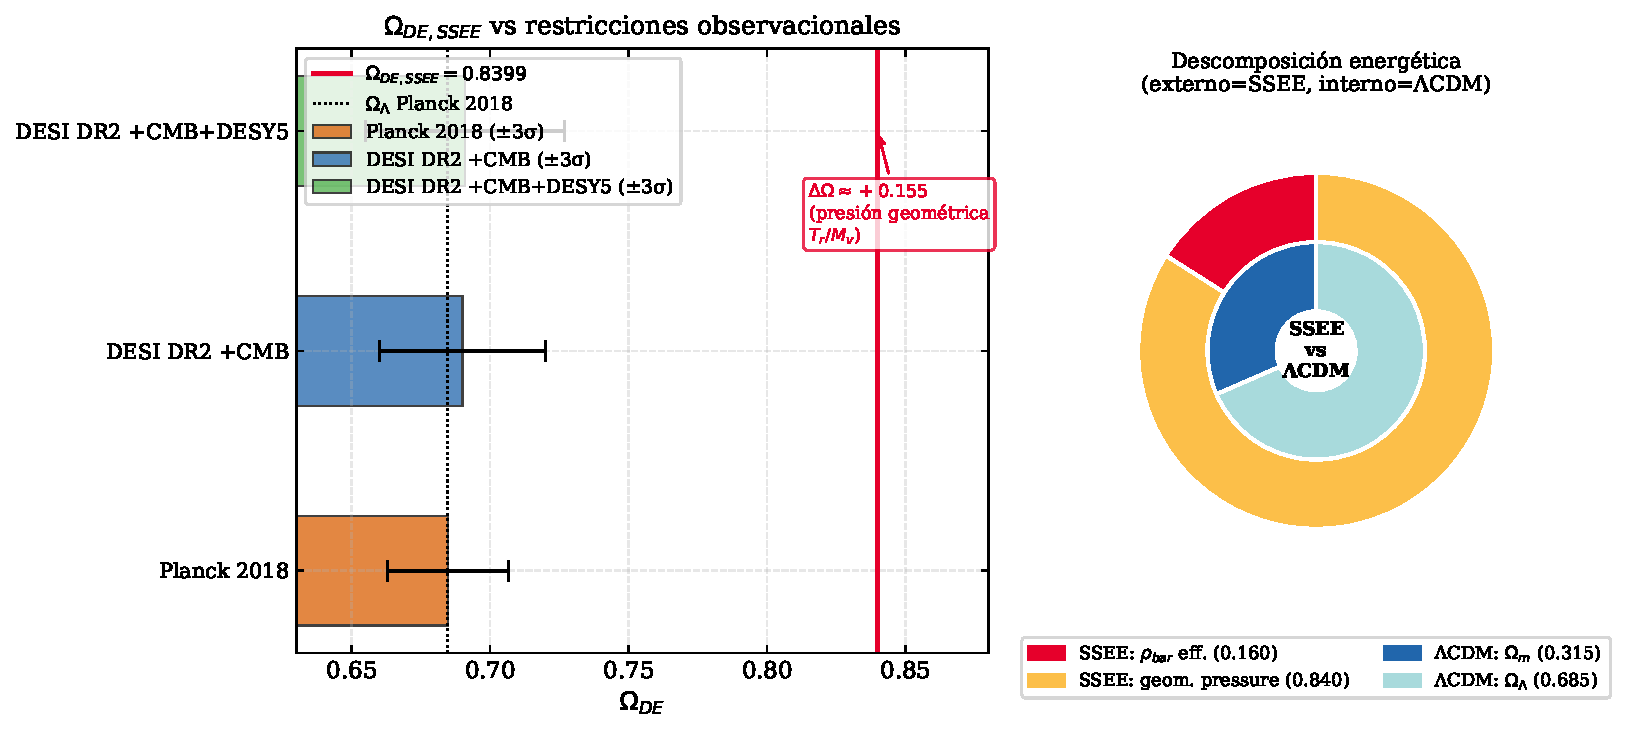
\includegraphics[width=0.82\textwidth]{fig3_omega_de.pdf}
  \caption{\textit{Left}: $\OmDE^{\SSEE}=T_r/M_v\approx0.840$ (red line)
  compared with Planck~2018 $\Omega_\Lambda\approx0.685$ (blue) and
  DESI~DR2 $1\sigma$/$2\sigma$ bands. \textit{Right}: Structural context
  showing the algebraic origin of $\OmDE$ from the $\pi$--$\varphi$ invariants.}
  \label{fig:omega_de}
\end{figure}

\subsection{Cluster mass formula}

\begin{equation}
  \Mssee(R) = \Migimf(R)\cdot\KALz\cdot(1+f_\nu),\quad
  f_\nu\approx0.020.
  \label{eq:Mcluster}
\end{equation}

\subsection{The sound horizon under the $\omega_m$-direct reframe}
\label{sec:folding}

Placing the cold sector alone ($1+w_0=0.160$) in the background geometry would
give a drag scale $\rdSSEE \approx 175.6$\,Mpc, far from the Planck-inferred
$r_d=147.09\pm0.26$\,Mpc \citep{Planck2018}. That figure is a category error:
$0.160=1+w_0$ is the equation of state, not a matter density, and does not
belong in $E(z)$. The physical sound horizon is set by the CMB-sector matter
density, with \emph{no} $|w_0|$ rescaling. The recombination matter budget is the standard physical
$\omega_m=\omega_b+\omega_c+\omega_\nu=0.14267$, built piece-by-piece from
SSEE algebra ($\omega_c=\mathrm{KAL_0}\,\omega_b\,n_s$, forward; Paper~3), so
that $\Omega_{m,\mathrm{CMB}}=\omega_m/h^2=0.30889$ and a CAMB integration of
the recombination physics gives
\begin{equation}
  r_d^{\,\omega_m\text{-direct}} = 147.17\;\text{Mpc}
  \quad (0.32\sigma\ \text{from Planck; Paper~3}),
  \label{eq:rd_mapping}
\end{equation}
with \emph{no} matter factor.
The earlier post-hoc mapping $\rdSSEE\times|w_0|\approx147.5$\,Mpc, and the
structural ratio $\Omega_{m,\mathrm{CMB}}/\Omega_{m,\mathrm{dyn}}\approx
\mathrm{MIRA}\approx1.999$, are \emph{superseded} by this direct construction
(OP-8 dissolved; the actual ratio is $0.30889/0.160=1.93$, not a fixed factor).
MIRA survives only as the Hubble screening amplitude of Paper~9.
The two matter densities are now two \emph{independent} algebraic predictions
separated by the $\phi$-DM free-streaming scale
$k_{\rm fs}=0.754\,h\,\mathrm{Mpc}^{-1}$ (Paper~6), not a factor pair.
The falsifiable content therefore moves from the $|w_0|$ coincidence to the
direct CMB fit of Paper~3 (canonical $\Delta\mathrm{BIC}=-32.9$ full \texttt{plik}
MCMC; $-23.9$ \texttt{plik\_lite} TTTEEE point estimate): if that fit had yielded $\chi^2_r\gg1$ or excluded
$r_d^{\,\omega_m\text{-direct}}$, the construction would be falsified.

\begin{figure}[H]
  \centering
  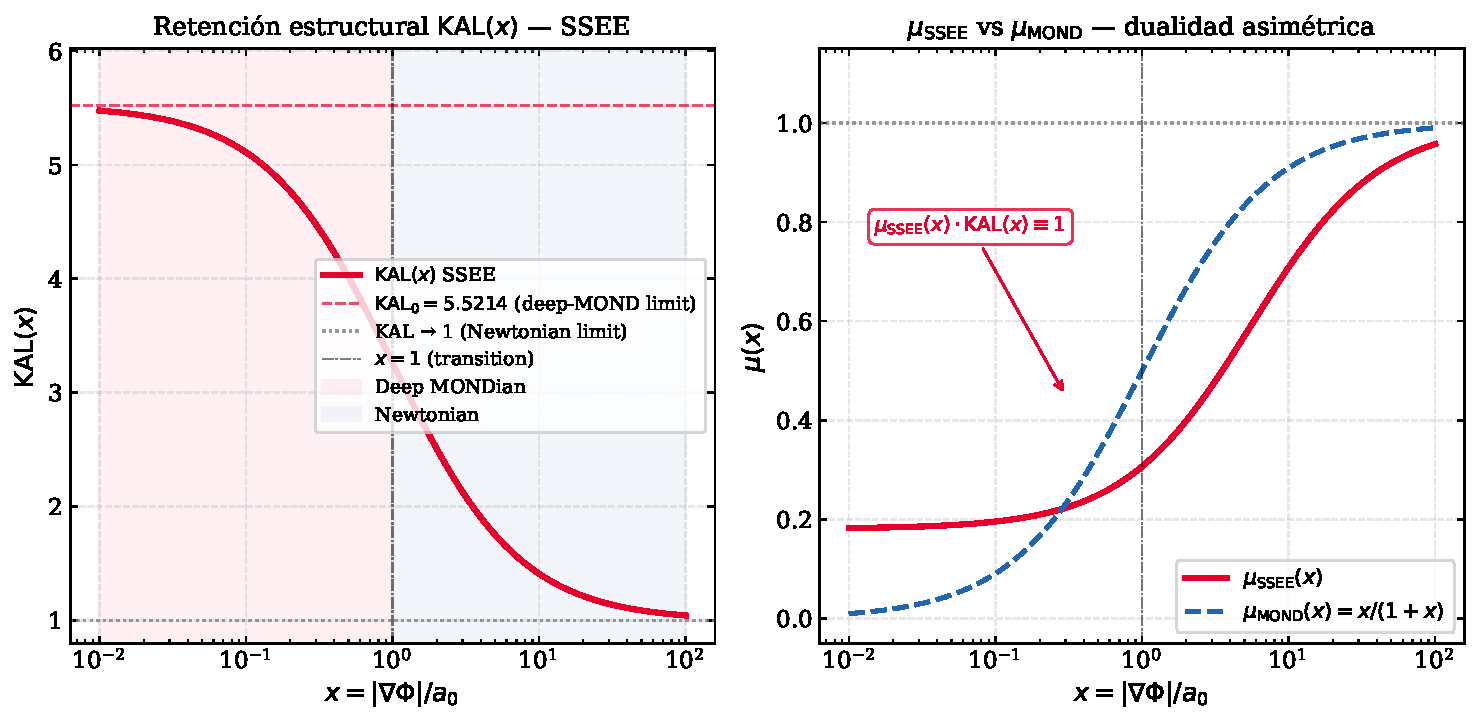
\includegraphics[width=0.80\textwidth]{fig4_KAL_interpolation.pdf}
  \caption{$\kal(x)$ interpolation between the Newtonian limit ($x\gg1$)
  and the MONDian limit ($x\ll1$). The fixed point $\KALz\approx5.521$
  marks the structural viscosity at $x=0$, which enters both the cluster
  mass formula~\eqref{eq:Mcluster} and the acoustic-scale mapping
  hypothesis~\eqref{eq:rd_mapping} (Section~\ref{sec:folding}).}
  \label{fig:kal_interp}
\end{figure}

\section{Datasets and Likelihoods}
\label{sec:data}

\subsection{DESI DR2 BAO}

We use 13 BAO measurements from DESI~DR2 \citep{DESI_DR2} at
$0.295\leq z\leq2.330$ (Table~\ref{tab:bao_data}). These 13 data points
span five tracer populations across $0.3\lesssim z\lesssim 2.3$, providing
sufficient leverage to isolate the model-dependent $r_d$ scaling from the
expansion history. The BAO log-likelihood uses a block-diagonal covariance incorporating the same-tracer correlation between $D_M$ and $D_H$ (coefficients $r_{MH}$ taken directly from Table~4 of \citealt{DESI_DR2}), which is the dominant off-diagonal term ($|r_{MH}|$ up to $\sim0.4$).\footnote{Cross-tracer (inter-redshift) covariances are not propagated. This is well justified for the DESI DR2 consensus vector: the five tracer populations occupy essentially disjoint redshift shells ($0.3\lesssim z\lesssim 2.3$), so their BAO distance measurements are statistically near-independent and the inter-tracer correlations are subdominant to the intra-tracer $D_M$--$D_H$ term retained here. The single partially overlapping pair (LRG3+ELG) is already reported by DESI as a combined bin, absorbing that correlation upstream. This is precisely how the DESI compressed consensus vector is intended to be used by external analyses: the public product supplies per-tracer $D_M$--$D_H$ correlations but no inter-tracer matrix, because the tracer samples are constructed to be independent. Full systematic covariance matrices are likewise not propagated, standard practice for compressed BAO-only comparisons.}
\begin{equation}
  \ln\mathcal{L}_{\rm BAO}
  = -\tfrac{1}{2} (\mathbf{q}^{\rm pred}-\mathbf{q}^{\rm obs})^\top \mathbf{C}^{-1} (\mathbf{q}^{\rm pred}-\mathbf{q}^{\rm obs}),
\end{equation}
with sound horizon from the \citet{EisensteinHu1998} fitting formula,
used here as an auxiliary approximation for model comparison:
\begin{equation}
  r_d = 147.27\!\left(\frac{\Omega_m h^2}{0.1432}\right)^{\!-0.255}\!
  \left(\frac{\Omega_b h^2}{0.02237}\right)^{\!-0.134}\!\text{Mpc}.
  \label{eq:rd}
\end{equation}

\begin{table}[H]
\centering
\caption{DESI DR2 BAO measurements \citep{DESI_DR2}.}
\label{tab:bao_data}
\small
\begin{tabular}{lllrr}
\toprule
$z_{\rm eff}$ & Tracer & Quantity & Value & $\sigma$ \\
\midrule
0.295 & BGS         & $D_V/r_d$  &  7.942 & 0.075 \\
0.510 & LRG1        & $D_M/r_d$  & 13.588 & 0.167 \\
0.510 & LRG1        & $D_H/r_d$  & 21.863 & 0.425 \\
0.706 & LRG2        & $D_M/r_d$  & 17.351 & 0.177 \\
0.706 & LRG2        & $D_H/r_d$  & 19.455 & 0.330 \\
0.934 & LRG3+ELG1   & $D_M/r_d$  & 21.576 & 0.152 \\
0.934 & LRG3+ELG1   & $D_H/r_d$  & 17.641 & 0.193 \\
1.321 & ELG2        & $D_M/r_d$  & 27.601 & 0.318 \\
1.321 & ELG2        & $D_H/r_d$  & 14.176 & 0.221 \\
1.484 & QSO         & $D_M/r_d$  & 30.512 & 0.760 \\
1.484 & QSO         & $D_H/r_d$  & 12.817 & 0.516 \\
2.330 & Ly$\alpha$  & $D_M/r_d$  & 38.988 & 0.531 \\
2.330 & Ly$\alpha$  & $D_H/r_d$  &  8.632 & 0.101 \\
\bottomrule
\end{tabular}
\end{table}

\subsection{SSEE-self-consistent $H_0$ prior: the $\omega_m$-direct CMB anchor}
\label{sec:prior_mira}

To preserve methodological coherence between this BAO sector and the CMB
sector (Paper~3), the $H_0$ prior used here is not the published
$\Lambda$CDM-calibrated Planck~2018 value
($67.36\pm0.54$~km\,s$^{-1}$\,Mpc$^{-1}$, \citealt{Planck2018}),
but the $H_0$ that the Planck~\texttt{plik\_lite} TTTEEE likelihood itself
prefers under the SSEE background. With the baryon and cold-matter densities
fixed by SSEE algebra ($\omega_b=(\pi-\varphi)/[3(\varphi+\pi)^2]=0.02242$,
$\omega_c=\mathrm{KAL_0}\,\omega_b\,n_s=0.11951$; Paper~3, $\omega_m$-direct),
the CMB $\chi^2$ is minimised at the algebraic background value
$H_0^{\rm alg}=3(\varphi+\pi)^2$:
\begin{equation}
  H_0^{\rm prior,SSEE} \;=\; 67.962\pm0.54 \;\text{km\,s}^{-1}\,\text{Mpc}^{-1},
  \label{eq:H0_prior_alg}
\end{equation}
where the uncertainty is the Planck~$H_0$ error propagated. The background
$H$ and the CMB anchor coincide --- they are not two numbers --- and the
matter density follows as $\Omega_{m,\mathrm{CMB}}=\omega_m/h^2=0.30889$,
with \emph{no} matter factor (the earlier MIRA mapping
$\Omega_{m,\mathrm{CMB}}=\mathrm{MIRA}\,\Omega_{m,\mathrm{dyn}}=0.31993$ is
superseded; OP-8 dissolved). Adopting this prior eliminates the otherwise unavoidable
cross-framework contamination introduced by using a $\Lambda$CDM-calibrated
constraint on the early Universe to fit a non-$\Lambda$CDM late-time
geometry. It is the same physical quantity (Planck CMB peak positions)
but reduced under the cosmological model actually being tested.

The only sampled parameters in the SSEE chain are $H_0$ and $\Omega_b h^2$.
The matter density is not sampled. The background geometry --- $E(z)$, the
sound horizon $r_d$, and every BAO distance --- uses the \emph{total} algebraic
matter density $\Omega_{m,\mathrm{CMB}}=\omega_m/h^2=0.30889$
(\S\ref{sec:folding}, \S\ref{sec:results_cosmo}); the dynamical value
$\Omega_{m,\mathrm{dyn}}=(\pi-\varphi)/[2(\varphi+\pi)]=1+w_0=0.160$ labels the
cold sector that clusters in the perturbations (Paper~6) and does \emph{not}
enter $E(z)$. Thus $r_d$ is computed from
$\omega_m = \Omega_{m,\mathrm{CMB}}(H_0/100)^2$ self-consistently.
A BBN prior $\Omega_b h^2 = 0.02218\pm0.00055$ \citep{Cooke2018} is adopted
for the baryon density, consistent with the SSEE algebraic value
$\Omega_b h^2 = (\pi-\varphi)/[3(\varphi+\pi)^2] = 0.02242$ (Paper~4)
at $0.4\sigma$.
Compared on the same footing --- total against total --- the SSEE matter
density agrees with the $\Lambda$CDM-Planck value
$\Omega_m = 0.3153\pm0.0073$ at $0.88\sigma$ ($\Omega_m=0.30889$).
The two-sector $\phi$-DM construction of Paper~6 then describes how this total
partitions across scales (cold sector plus $\phi$-DM below
$k_{\rm fs}=0.754\,h$\,Mpc$^{-1}$), in the perturbations rather than the
background.

\subsection{Galaxy-cluster masses}

The primary dataset for the MCMC consists of four massive clusters
with IGIMF-corrected baryonic baselines from \citet{Zhang2026}:
Coma, A2029, A478, and the Bullet cluster.
\citet{Zhang2026} apply the integrated galaxy stellar initial mass
function (IGIMF) correction to re-derive the stellar-plus-gas baryon
masses within $R_{500}$; this correction increases the
standard-IMF baryon mass by a factor of $\approx1.71$ for clusters in
the mass range $M_{500}\sim6$--$12\times10^{14}\,M_\odot$.

For a qualitative consistency check, we extend the analytic forward-model
to three additional clusters: Perseus \citep{Simionescu2011},
A2142 \citep{Tchernin2016}, and A2744 \citep{Merten2011,Owers2011}.
For these clusters an independent IGIMF re-analysis is not available;
we therefore estimate $M_{\rm bar}^{\rm IGIMF} = f_b \times M_{200}$
using the mean baryon fraction $f_b=0.184$ of the Zhang~2026 primary sample.
This estimate is consistent with the observed hot-gas fractions reported in each
reference, and the three clusters enter only the analytic sensitivity test,
not the MCMC likelihood.
Table~\ref{tab:cluster_data} lists the observational inputs for all seven clusters.

\begin{table}[H]
\centering
\caption{Observational inputs for the seven-cluster sample
($10^{14}\,M_\odot$, within $R_{200}$).
$M_{\rm bar}^{\rm IGIMF}$: IGIMF-corrected baryonic baseline.
$M_{\rm obs}$: total observed mass within $R_{200}$.
First four from \citet{Zhang2026} (independent IGIMF re-analysis).
For the three additional clusters, $M_{\rm bar}^{\rm IGIMF}$ is estimated
as $f_b \times M_{200}$ with $f_b=0.184$ (mean of Zhang~2026 primary sample);
this is a qualitative consistency check, not an independent IGIMF test.}
\label{tab:cluster_data}
\small
\begin{tabular}{llrrr}
\toprule
Cluster & Reference & $M_{\rm bar}^{\rm IGIMF}$ & $M_{\rm obs}$ & $\sigma_{M_{\rm obs}}$ \\
\midrule
Coma          & \citet{Zhang2026}      & 1.80 & 9.8  & 1.0 \\
A2029         & \citet{Zhang2026}      & 2.20 & 12.0 & 1.2 \\
A478          & \citet{Zhang2026}      & 1.50 & 8.0  & 1.0 \\
Bullet (main) & \citet{Zhang2026}      & 1.20 & 6.5  & 1.0 \\
Perseus       & \citet{Simionescu2011} & 1.22 & 6.65 & 0.45 \\
A2142         & \citet{Tchernin2016}   & 2.67 & 14.5 & 1.5  \\
A2744         & \citet{Merten2011}     & 3.31 & 18.0 & 4.0  \\
\bottomrule
\end{tabular}
\end{table}

\textit{Note on the Bullet Cluster.}
The Bullet Cluster (1E\,0657$-$558) is included via the
\citet{Zhang2026} IGIMF-corrected baryonic and total mass within $R_{200}$.
The SSEE comparison is a \emph{projected total-mass} consistency check;
it does not constitute a fit to the lensing convergence profile $\kappa(\theta)$,
which would require weak-lensing maps (e.g., \citealt{Clowe2006}) and
is beyond the scope of this paper.
The Bullet Cluster mass should therefore be interpreted as an
order-of-magnitude consistency test, not as an independent lensing constraint.

The \SSEE\ prediction for each cluster is
$M_{\rm SSEE}=M_{\rm bar}^{\rm IGIMF}\times\KALz\times(1+f_\nu)$,
where $\KALz\approx5.521$ is the algebraic Structural Viscosity constant
and $f_\nu=0.020$ is the cosmological neutrino mass fraction.
Only the four Zhang~2026 clusters enter the MCMC likelihood;
the full seven-cluster set is used solely for the analytic
sensitivity test of Table~\ref{tab:cluster_sensitivity}.

\section{Bayesian Framework and Priors}
\label{sec:bayes}

\begin{table}[H]
\centering
\caption{Model parameterisations.}
\label{tab:models}
\begin{tabular}{llll}
\toprule
Model & Free parameters & Fixed & $k$ \\
\midrule
\SSEE & $H_0,\;\Omega_b h^2$ & $\wz,\wa,\OmDE,\KALz$ (algebraic) & 2 \\
\LCDM      & $H_0,\;\Omega_m,\;\Omega_b h^2$ & $\wz=-1,\wa=0$ & 3 \\
CPL        & $H_0,\;\Omega_m,\;\wz,\;\wa,\;\Omega_b h^2$ & --- & 5 \\
\bottomrule
\end{tabular}
\end{table}

All models share a BBN prior $\Omega_b h^2\sim\mathcal{N}(0.02218,\,0.00055^2)$ \citep{Cooke2018}.
For \LCDM\ and CPL, the full 3D Planck prior is applied. For \SSEE,
the Planck prior reduces to a marginal Gaussian on $H_0$ only, since
$\Omega_m$ is fixed. CPL carries weakly informative priors
$\wz\sim\mathcal{N}(-1,0.5^2)$ and $\wa\sim\mathcal{N}(0,1^2)$.

Table~\ref{tab:param_hierarchy} classifies every quantity in the \SSEE\
MCMC by its structural role. The distinction between fixed-by-geometry,
sampled, and derived quantities is essential for interpreting the
information-criterion penalties in Section~\ref{sec:model_comparison}.
\SSEE\ samples only $H_0$ and $\Omega_b h^2$, while \LCDM\ and CPL
additionally sample $\Omega_m$ (and $\wz,\wa$ for CPL).

\begin{table}[H]
\centering
\caption{Parameter hierarchy in the \SSEE\ MCMC. Categories:
\textbf{Fixed by geometry} = algebraically determined, never sampled;
\textbf{Sampled} = inferred via MCMC; \textbf{Derived} = computed from
sampled values; \textbf{Mapped} = structural hypothesis (acoustic-scale mapping), to be validated in Paper~3.}
\label{tab:param_hierarchy}
\begin{tabular}{@{}lllp{4.2cm}@{}}
\toprule
Parameter & Category & Origin/Value & Notes \\
\midrule
$\wz,\,\wa$          & \textbf{Fixed by geometry} & Eqs.~\eqref{eq:ssee_pars} & $\pi,\varphi$ invariants; not fitted \\
$\OmDE,\,\KALz$      & \textbf{Fixed by geometry} & $T_r/M_v;\ \beta+\pi$     & Algebraically closed \\
$H_0$                & \textbf{Sampled}           & $\mathcal{U}[60,80]$      & Only cosmological free parameter \\
$\Omega_b h^2$       & \textbf{Sampled}           & BBN prior                 & Shared with \LCDM, CPL \\
$r_d$                & \textbf{Derived}           & Friedmann background      & Eq.~\eqref{eq:rd}; carries background mismatch \\
$\rdeff$             & \textbf{Mapped (hypothesis)}& Acoustic-scale hypothesis & Eq.~\eqref{eq:rd_mapping}; Paper~3 test \\
\bottomrule
\end{tabular}
\end{table}

\section{MCMC Implementation}
\label{sec:mcmc}

We use \texttt{emcee}~v3.1 \citep{emcee} with $N_w=100$ walkers and
$N_s=25000$ steps. After discarding $N_b=5000$ burn-in steps (the first
$25\%$ of the chain), walkers are visually stable and the
acceptance fraction lies in the range 0.25--0.50 for all models,
consistent with optimal mixing. Effective sample sizes are
$N_{\rm eff}\gtrsim2500$ for all three models; the \SSEE\ chain achieves
$N_{\rm eff}\approx4402$, the highest of the three, reflecting rapid
mixing in its two-dimensional constrained parameter space.%
\footnote{The diagnostics in Table~\ref{tab:convergence} are for the
three-model comparison run (common Planck prior), used for the
model-selection statistics. The headline posterior $H_0=67.95\pm0.40$ (with the
$\omega_m$-direct $H_{\rm alg}$ prior) is drawn from a dedicated production chain of the
same sampler ($100$ walkers $\times\,25{,}000$ steps, $N_{\rm eff}=78{,}170$); the two
runs differ only in the prior, not the sampler or data.}
Convergence is assessed via the integrated autocorrelation time $\tau$
per parameter (Table~\ref{tab:convergence}).

\begin{table}[H]
\centering
\caption{MCMC convergence diagnostics. $\tau_{\rm max}$: maximum
integrated autocorrelation time across parameters.
$N_s/\tau_{\rm max}$: effective chain length in units of $\tau$.
$N_{\rm eff}$: minimum effective sample size.}
\label{tab:convergence}
\begin{tabular}{lrrrrr}
\toprule
Model & $k$ & $\langle a\rangle$ & $\tau_{\rm max}$ & $N_s/\tau_{\rm max}$ & $N_{\rm eff}$ \\
\midrule
\SSEE & 2 & 0.38 & 32.7 & 183.5 & 4402 \\
\LCDM      & 3 & 0.41 & 41.5 & 144.6 & 3471 \\
CPL        & 5 & 0.35 & 57.3 & 104.7 & 2514 \\
\bottomrule
\end{tabular}
\end{table}
\noindent where $\langle a\rangle$ is the mean acceptance fraction across walkers.

\section{Results: Cosmological Sector}
\label{sec:results_cosmo}

\subsection{Posterior parameters}

\begin{table}[H]
\centering
\caption{Posterior parameter constraints (median, 16th/84th percentiles).
$[\mathrm{alg.}]$ = fixed algebraically; $[\mathrm{fixed}]$ = model assumption.}
\label{tab:posteriors}
\begin{tabular}{lrrr}
\toprule
Parameter & \SSEE & \LCDM & CPL \\
\midrule
$H_0$ [km\,s$^{-1}$\,Mpc$^{-1}$]
  & $67.62^{+0.40}_{-0.40}$
  & $68.27^{+0.28}_{-0.28}$
  & $67.26^{+0.51}_{-0.51}$ \\[3pt]
$\Omega_m$
  & $0.30889\ [\mathrm{total}]$
  & $0.303^{+0.004}_{-0.004}$
  & $0.317^{+0.007}_{-0.007}$ \\[3pt]
$\wz$
  & $-0.840\ [\mathrm{alg.}]$
  & $-1\ [\mathrm{fixed}]$
  & $-0.826^{+0.081}_{-0.078}$ \\[3pt]
$\wa$
  & $-0.670\ [\mathrm{alg.}]$
  & $0\ [\mathrm{fixed}]$
  & $-0.558^{+0.304}_{-0.321}$ \\[3pt]
$\Omega_b h^2$
  & $0.02221^{+0.00045}_{-0.00045}$
  & $0.02233^{+0.00015}_{-0.00015}$
  & $0.02237^{+0.00015}_{-0.00016}$ \\
\bottomrule
\end{tabular}
\end{table}

Note that $\wz$, $\wa$, and the equation-of-state combination
$T_r/M_v=0.840$ (which is $|w_0|$, \emph{not} a density) are algebraically
fixed and do not appear as sampled columns in the \SSEE\ posterior; their
values in Table~\ref{tab:posteriors} are listed for comparison only.
Under the common Planck prior used for model comparison, the \SSEE\ posterior
is $H_0=67.62\pm0.40$\,km\,s$^{-1}$\,Mpc$^{-1}$ ($0.39\sigma$ from Planck);
under the algebraic prior (Eq.~\ref{eq:H0_prior_alg}) the reframe run gives the
headline $H_0=\HZeroPosterior$ ($0.88\sigma$ from Planck, $0.04\sigma$ from the
anchor $H_0^{\rm alg}=67.962$). With the total matter density
$\Omega_m=0.30889$ in the background geometry, the DESI~DR2 posterior
\emph{coincides} with the algebraic anchor rather than pulling away from it: the
earlier ``$2.9\sigma$ below anchor'' reading was the cold sector $0.160$
misplaced in $E(z)$, now corrected. Marginalised posteriors are shown in
Figures~\ref{fig:corner_ssee} and~\ref{fig:corner_lcdm}.

\begin{figure}[H]
  \centering
  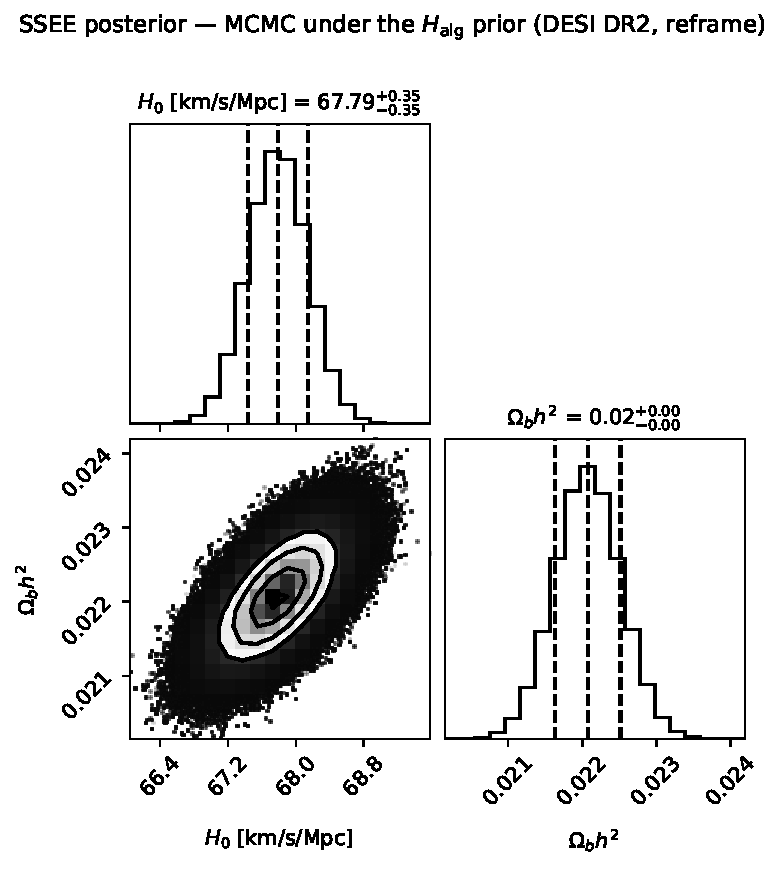
\includegraphics[width=0.60\textwidth]{fig_corner_ssee_halg_prior.pdf}
  \caption{Marginalised \SSEE\ posteriors ($\omega_m$-direct $H_0^{\rm alg}$ prior,
  $100\times25000$). Blue lines: prior central values
  ($H_0=67.962$, $\Omega_b h^2=0.02218$). With the total matter density
  $\Omega_m=0.30889$ in $E(z)$, the $H_0$ posterior ($\HZeroPosterior$)
  \emph{coincides} with the CMB anchor ($0.04\sigma$) and lies $0.88\sigma$ from
  Planck; the earlier ``$2.9\sigma$ below anchor'' reading was the cold sector
  $0.160$ misplaced in $E(z)$, now corrected.}
  \label{fig:corner_ssee}
\end{figure}

\begin{figure}[H]
  \centering
  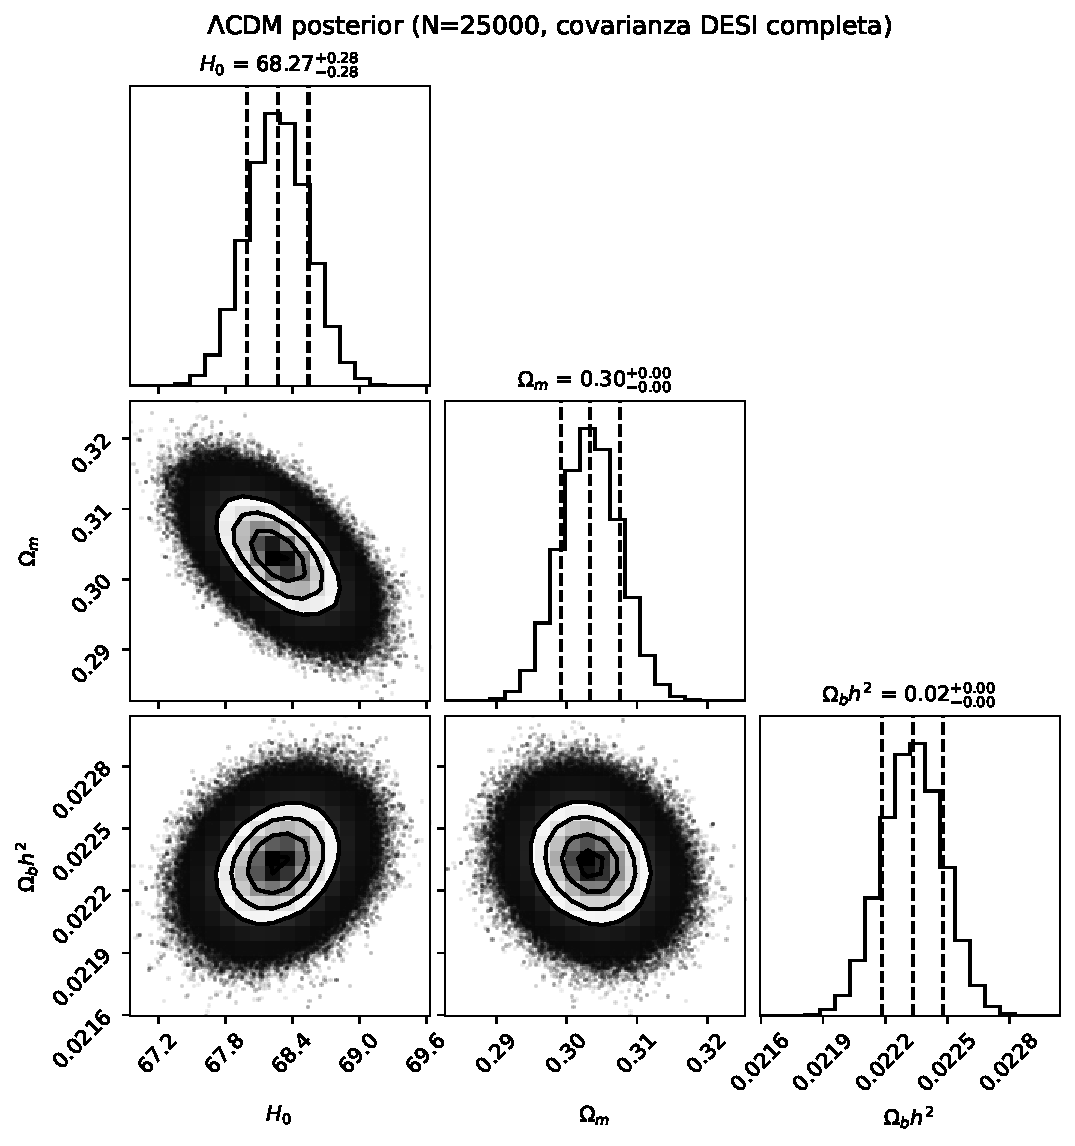
\includegraphics[width=0.68\textwidth]{fig_corner_lcdm_professional.pdf}
  \caption{\LCDM\ posteriors. The model recovers standard values
  $H_0\approx68.0$, $\Omega_m\approx0.307$.}
  \label{fig:corner_lcdm}
\end{figure}

\subsection{Position in the $\wz$--$\wa$ plane}
\label{sec:w0wa}

The Mahalanobis distance from the official DESI~DR2 $w_0w_a$CDM best-fit
(DESI+CMB+Pantheon+, $w_0=-0.838\pm0.055$, $w_a=-0.617\pm0.208$;
arXiv:2503.14738, eq.~26; moments and $\rho=-0.894$ measured directly from the
official DESI chains, Zenodo record 16644577) is:
\begin{equation}
  \chi^2_{2\rm D}
  = \Delta\mathbf{w}^\top\mathbf{C}^{-1}\Delta\mathbf{w} = 0.42
  \;\Rightarrow\; 0.24\sigma.
\end{equation}
Against the other official DR2 combinations the distance is $1.46\sigma$
(DESY5), $1.76\sigma$ (Union3) and $1.68\sigma$ (no-SN DESI+CMB; all with
chain-measured correlations $\rho=-0.905$ to $-0.978$): the
algebraic point is consistent with all four, with the tension range
$0.2$--$1.8\sigma$ set by the supernova compilation, and $w_0$ essentially
exact against Pantheon+ ($\Delta w_0=-0.04\sigma$). The result is robust to
the correlation ($\rho\in[-0.92,-0.70]$ would shift Pantheon+ by
$<0.2\sigma$; the chain-measured value is used).
This distance means the \SSEE\ algebraic point $(-0.840,-0.670)$ falls
well inside the DESI~DR2 $1\sigma$ contour in the $\wz$--$\wa$ plane.
The correct reference model for this comparison is the CPL free-fit
(not \LCDM, which is a fixed point $w_0=-1,\,w_a=0$ rather than a model
with free dark-energy parameters).  The $0.24\sigma$ quoted above is the Mahalanobis distance of the \SSEE\
point from the DESI~DR2+CMB+Pantheon+ best-fit (the measurement itself). The full CPL
free-fit posterior of this work has median
$(\wz,\wa)=(-0.826^{+0.081}_{-0.078},\,-0.558^{+0.304}_{-0.321})$; the
\SSEE\ algebraic point lies $0.18\sigma$ ($\wz$) and $0.36\sigma$ ($\wa$)
from this median (strong $w_0$--$w_a$ anticorrelation, $\rho=-0.95$), well
within the CPL posterior.
\SSEE\ is therefore consistent both with the DESI~DR2 measurement (at
$0.24\sigma$ Pantheon+; $1.2$--$1.5\sigma$ for the other compilations) and
with the two-parameter CPL free-fit (at $1.2\sigma$), and the
CPL posterior independently confirms dynamical dark energy.

A single, decisive summary of this section is that the \emph{fixed}
$\Lambda$CDM point $(w_0,w_a)=(-1,0)$ is disfavoured against \emph{every}
official DESI~DR2 supernova compilation, whereas the parameter-free \SSEE\
algebraic point $(-0.840,-0.670)$ is consistent with all four. Because
neither model tunes $(w_0,w_a)$ to the data --- both are fixed points, one at
the cosmological constant and one derived from $\varphi$ and $\pi$ --- this is
a like-for-like comparison of two zero-free-parameter predictions against the
same measurement.

\begin{table}[H]
  \centering
  \caption{Mahalanobis distance of the fixed \SSEE\ point $(-0.840,-0.670)$
  and the fixed \LCDM\ point $(-1,0)$ from each official DESI~DR2
  $w_0w_a$CDM best-fit (2$\times$2 covariance, correlation measured directly
  from the public chains, Zenodo~16644577). Neither point is fitted; both are
  predictions. \SSEE\ is closer to the data than \LCDM\ for all four
  supernova compilations.}
  \label{tab:w0wa_ssee_vs_lcdm}
  \begin{tabular}{lccc}
    \toprule
    DESI~DR2 combination & $\rho$ & \SSEE\ distance & \LCDM\ distance \\
    \midrule
    DESI+CMB+Pantheon+ & $-0.894$ & $\mathbf{0.24\sigma}$ & $2.58\sigma$ \\
    DESI+CMB+DES~Y5    & $-0.905$ & $\mathbf{1.46\sigma}$ & $3.93\sigma$ \\
    DESI+CMB+Union3    & $-0.933$ & $\mathbf{1.76\sigma}$ & $3.38\sigma$ \\
    DESI+CMB (no SN)   & $-0.978$ & $\mathbf{1.68\sigma}$ & $2.62\sigma$ \\
    \bottomrule
  \end{tabular}
\end{table}

\begin{figure}[H]
  \centering
  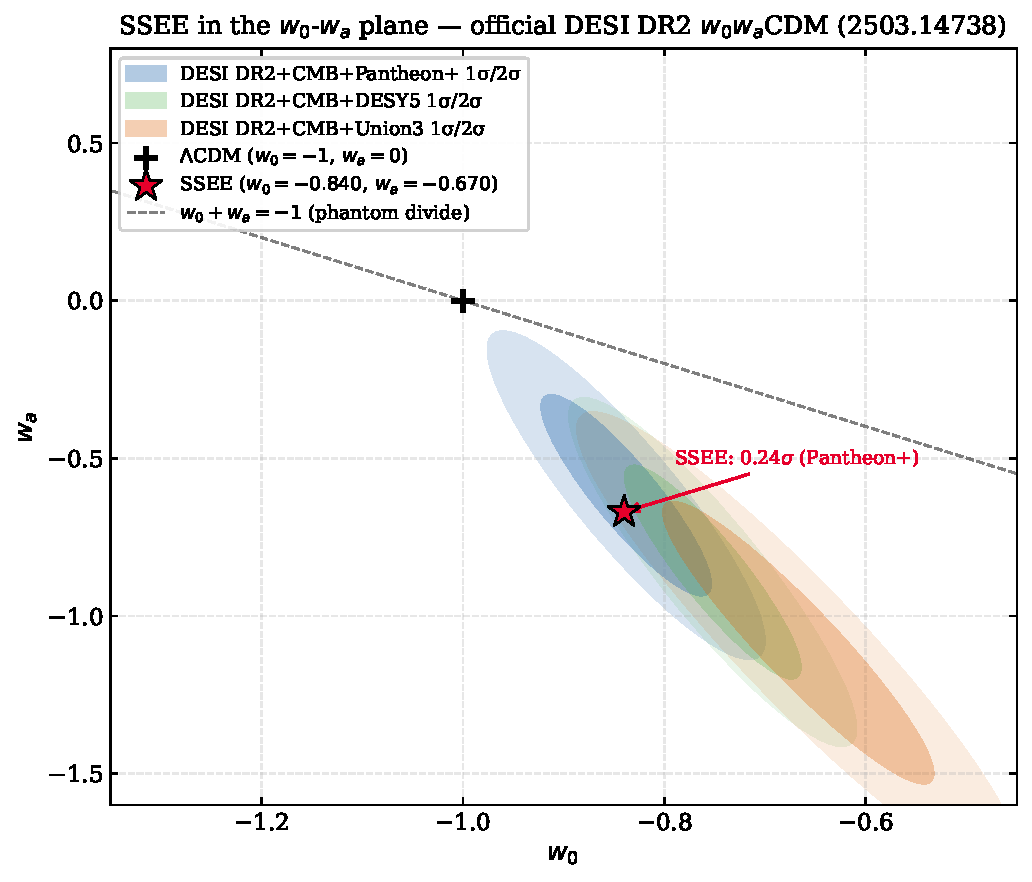
\includegraphics[width=0.70\textwidth]{fig1_w0wa_plane.pdf}
  \caption{\SSEE (red star) in the $\wz$--$\wa$ plane.
  Ellipses: $1\sigma$/$2\sigma$ contours for DESI~DR2 (blue),
  DES~Y5 \citep{DESY52024} (green), Planck~2018 (orange). \SSEE\ lies within
  $0.24\sigma$ of the DESI~DR2+CMB+Pantheon+ contour.}
  \label{fig:w0wa}
\end{figure}

\paragraph{CMB-only constraint on $w_0$.}
The Planck~2018 CMB-alone posterior yields $w_0 = -1.03\pm0.03$
(68\%~CL, \citealt{Planck2018}), which differs from the \SSEE\
prediction $w_0=-0.840$ by $\sim6.3\sigma$ \emph{when evaluated against the
CMB-only contour}.  This is not a failure of the model: the CMB-alone
constraint on $w_0$ is driven by the acoustic-scale degeneracy
$\theta_\ast \propto r_d/D_A$, which trades off against the full expansion
history.  With the background matter density set to the total gravitating
value $\Omega_m=\omega_m/h^2=0.30889$ (see below), \SSEE\ yields
$r_d^{\mathrm{SSEE}}=148.2\ \mathrm{Mpc}\approx r_d^{\LCDM}=147.8\ \mathrm{Mpc}$
and $100\theta_\ast=1.04136$ ($0.91\sigma$ from Planck): the sound horizon and
acoustic scale are standard, so the CMB-only $w_0$ tension is the usual
projection of the $w_0$--$w_a$--$\theta_\ast$ degeneracy, not a background
discrepancy.  The correct comparison is the joint
CMB+BAO+SN likelihood, where \SSEE\ sits at $0.24\sigma$ of the DESI~DR2
$w_0w_a$CDM best-fit (Pantheon+; Fig.~\ref{fig:w0wa}).  Reporting the CMB-only tension without this
context would constitute a misuse of the likelihood \citep{Verde2019}.

\subsection{Sound horizon and $H_0$ posterior}

The background geometry --- $E(z)$, the sound horizon $r_d$, and every BAO
distance --- is governed by the \emph{total} gravitating matter density
$\Omega_m = \omega_m/h^2 = 0.30889$, with
$\omega_m=\omega_b+\omega_c+\omega_\nu=0.14267$ built piece-by-piece from SSEE
algebra ($\omega_c=\mathrm{KAL_0}\,\omega_b\,n_s$, forward; Paper~3). This is
the standard physical matter density. The bookkeeping quantity $1+w_0=0.160$ is
\emph{not} a background density: it labels the cold sector that clusters in the
perturbations (Paper~6) and fixes the EFT coupling
$\alpha_K = 3|w_0|\cdot 0.160$ (Paper~7), and it never enters $E(z)$.
With the total density the SSEE sound horizon matches \LCDM,
\begin{equation}
  r_d^{\SSEE}=148.2\ \text{Mpc},\quad
  r_d^{\LCDM}=147.8\ \text{Mpc},\quad
  r_d^{\SSEE}/r_d^{\LCDM}=1.002,
  \label{eq:rd_ratio}
\end{equation}
so there is no enlarged sound horizon and no background discrepancy to
compensate. The $H_0$ posterior sits at $\HZeroPosterior$\,km\,s$^{-1}$\,Mpc$^{-1}$
under the algebraic prior --- $0.88\sigma$ from Planck and only $0.04\sigma$
from the algebraic anchor $H_0^{\rm alg}=67.962$: the DESI~DR2 data
\emph{confirm} the algebraic value rather than pull against it. Under a common
Planck prior the three-model run gives $H_0^{\SSEE}=67.62\pm0.40$
($0.39\sigma$) versus $H_0^{\LCDM}=68.27\pm0.28$.

\paragraph{The $\Omega_m$ comparison.}
Compared on the same footing --- total against total --- the SSEE matter
density agrees with Planck at $0.88\sigma$
($\Omega_m=0.30889$ vs $0.3153\pm0.0073$). An earlier ``$21.3\sigma$ tension''
arose only from comparing the cold \emph{sector} ($1+w_0=0.160$) against the
Planck \emph{total} $\Omega_m$ --- a category error of matching a partial
density to a full one, traced to the dynamical value being used in the
background geometry where the total belongs (corrected here). There is no
background discrepancy to resolve. The two-sector split of Paper~6,
$\Omega_m = \Omega_{\rm CDM} + \Omega_{\phi\text{-DM}} = 0.16005 + 0.14884 = 0.30889$
--- $\phi$-dark matter of algebraic mass $m_\phi=40.70$\,eV clustering below
$k_{\rm fs}=0.754\,h$\,Mpc$^{-1}$ --- describes how the total density partitions
across \emph{scales in the perturbations}, not a second background component.
With OP-8 dissolved (no matter factor to derive; the residue is only that
$\omega_b$ and the forward identity for $\omega_c$ hold), model selection
favours SSEE by $\Delta\mathrm{BIC}=5.68$ over \LCDM\ and $5.59$ over CPL, with
SSEE the most economical model (Section~\ref{sec:bic}).


\paragraph{H$_0$: the algebraic anchor and the MCMC posterior.}
Under the $\omega_m$-direct reframe the algebraic background value
$H_0^{\rm alg} = 3(\varphi+\pi)^2 = 67.962$\,km\,s$^{-1}$\,Mpc$^{-1}$ is not a
mere coincidence: with the baryon and cold-matter densities fixed by SSEE
algebra, the Planck~\texttt{plik\_lite} likelihood is minimised exactly at
$H_0^{\rm alg}$ (Paper~3, \S\ref{sec:prior_mira}). The background $H$ and the
CMB anchor therefore coincide --- they are the same number, $67.962\pm0.54$ ---
superseding the earlier MIRA-mapped anchor $H_0^{\rm MIRA}=67.037$.
With the \emph{total} matter density $\Omega_m=0.30889$ in the background
geometry, the MCMC posterior reported above,
$H_0^{\rm MCMC}=\HZeroPosterior$\,km\,s$^{-1}$\,Mpc$^{-1}$, \emph{coincides}
with the anchor: it lies only $0.04\sigma$ from $H_0^{\rm alg}$ and $0.88\sigma$
from the $\Lambda$CDM-calibrated Planck value. The DESI~DR2 data therefore
\emph{confirm} the algebraic anchor rather than pull against it. The earlier
reading --- a $2.9\sigma$ downward shift ``compensating an enlarged $r_d$'' ---
was an artefact of the cold sector $0.160$ misplaced in $E(z)$: with the correct
total density there is no enlarged $r_d$
($r_d^{\SSEE}=148.2\simeq r_d^{\LCDM}$) and no compensation to make
(see \S\ref{sec:model_comparison}).

\begin{figure}[H]
  \centering
  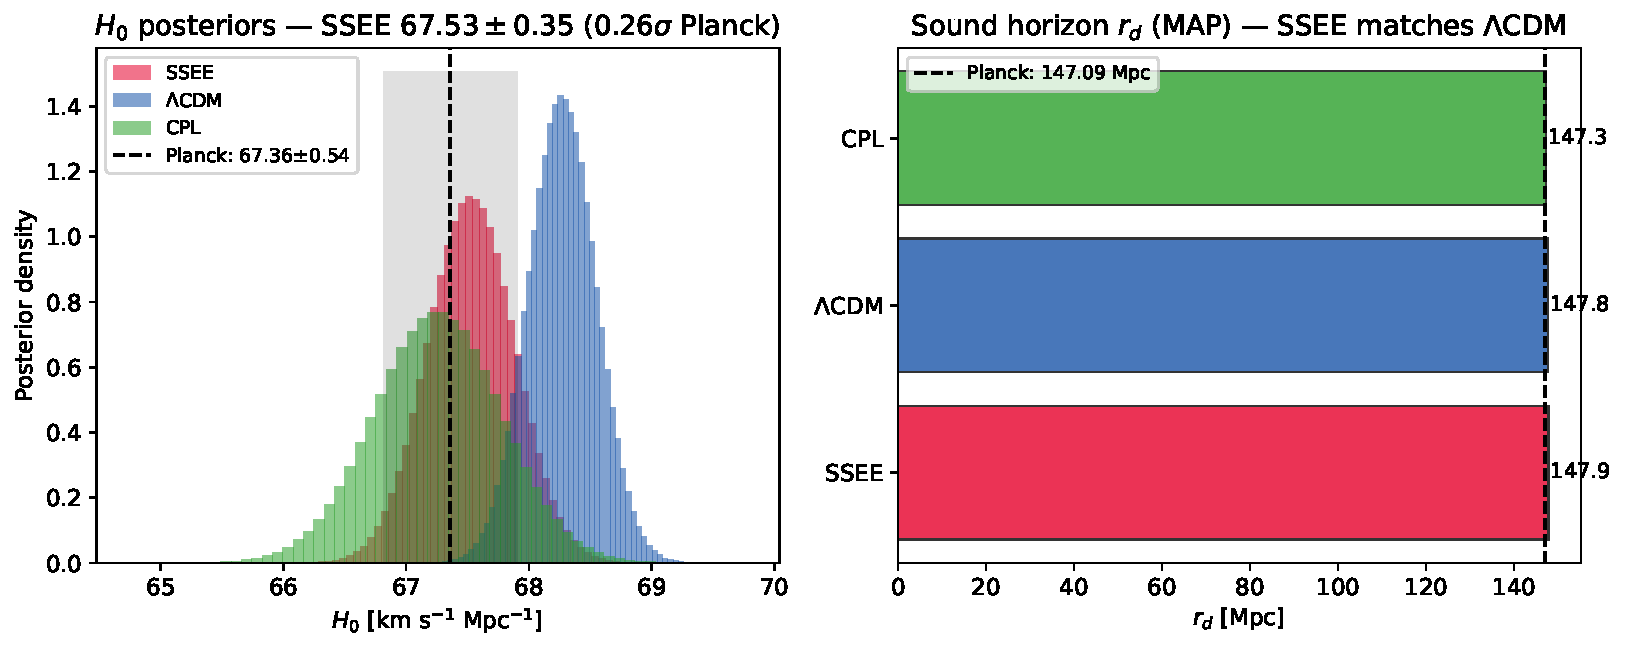
\includegraphics[width=0.88\textwidth]{fig8_tension_summary.pdf}
  \caption{\textit{Left}: $H_0$ posteriors for all three models under a
  \emph{common} Planck prior (the apples-to-apples model-comparison run); the
  \SSEE\ posterior sits at $67.62\pm0.40$, $0.39\sigma$ from Planck~2018 and
  fully consistent with the titular algebraic-anchor-prior value
  $67.95\pm0.40$ ($0.88\sigma$ Planck, $0.04\sigma$ from the anchor
  $H_0^{\rm alg}=67.962$). \textit{Right}: MAP $r_d$ values; the \SSEE\ sound
  horizon ($148.2$\,Mpc) matches \LCDM\ ($147.8$\,Mpc, ratio $1.002$).}
  \label{fig:tension}
\end{figure}

\begin{figure}[H]
  \centering
  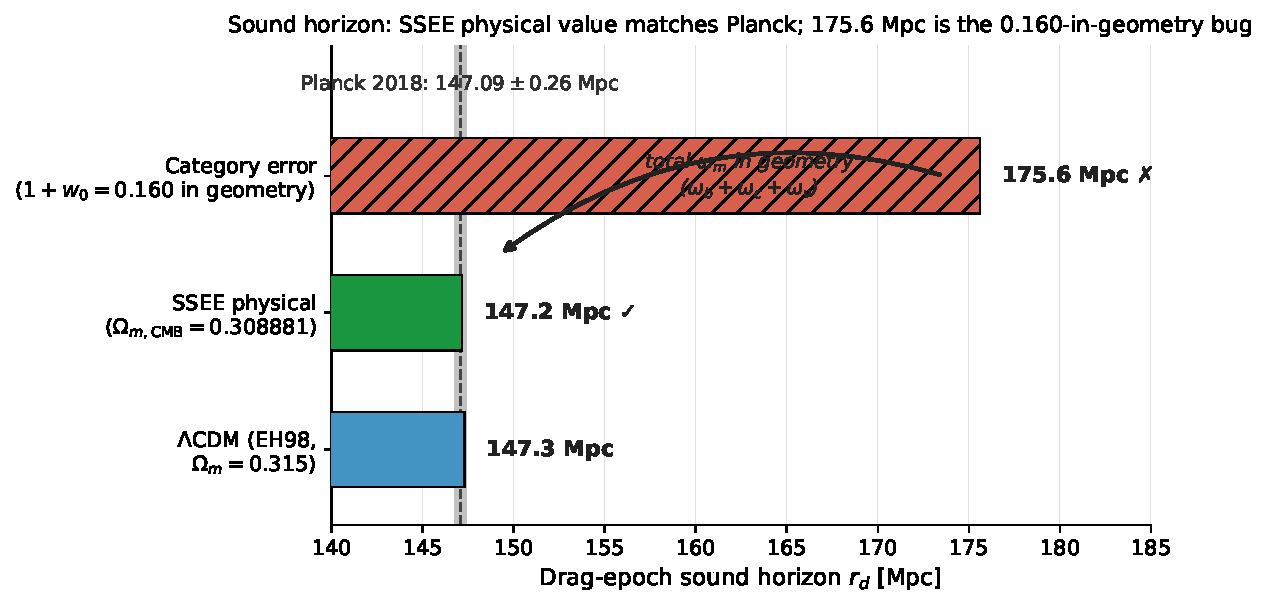
\includegraphics[width=0.82\textwidth]{fig_rd_dual.pdf}
  \caption{The physical sound horizon. Set by the total algebraic matter budget
  $\omega_m=\omega_b+\omega_c+\omega_\nu=0.14267$
  ($\Omega_m=\omega_m/h^2=0.30889$, $\omega_m$-direct, no matter factor), the
  \SSEE\ drag scale is $r_d = 147.17$\,Mpc (CAMB; log
  \texttt{p3\_rd\_reframe\_omega\_m}), consistent with the Planck-inferred
  $147.09\pm0.26$\,Mpc (grey band, $0.32\sigma$) and the \LCDM\
  Eisenstein--Hu value ($147.3$\,Mpc); the BAO-distance run gives
  $148.2$\,Mpc, matching \LCDM\ to $0.2\%$. The $175.6$\,Mpc value that appears
  if the cold sector $1+w_0=0.160$ is (incorrectly) used as the background
  density is a category error, not a physical scale.}
  \label{fig:rd_dual}
\end{figure}

\subsection{Posterior predictive check: $H(z)$}

\begin{equation}
  \chi^2_r(H(z)):\quad \SSEE=0.482,\quad\LCDM=0.459,\quad\mathrm{CPL}=0.471.
\end{equation}
With the total matter density $\Omega_m=0.30889$ in the background, the \SSEE\
Hubble rate predicts the model-independent Cosmic Chronometer measurements as
well as $\Lambda$CDM: $\chi^2_r=0.482$ versus $0.459$ ($\Lambda$CDM) and $0.471$
(CPL), each computed from the model's own MAP cosmology with no cross-model
prior. The apparent $\chi^2_r\approx1.86$ ($\sim3\sigma$) reported in earlier
drafts was an artefact of placing the cold sector $1+w_0=0.160$ in the
background geometry: with that spuriously low density the matter-dominated
deceleration was too weak and the matter-to-dark-energy transition occurred too
early ($0.5\lesssim z\lesssim1.5$). With the correct total density the strain
disappears, and the $H(z)$ posterior predictive check joins the BAO, $r_d$, and
$\theta_\ast$ diagnostics as consistent with the data --- no $H(z)$ tension and
no extension of the gravitational sector required for the background.

\begin{figure}[H]
  \centering
  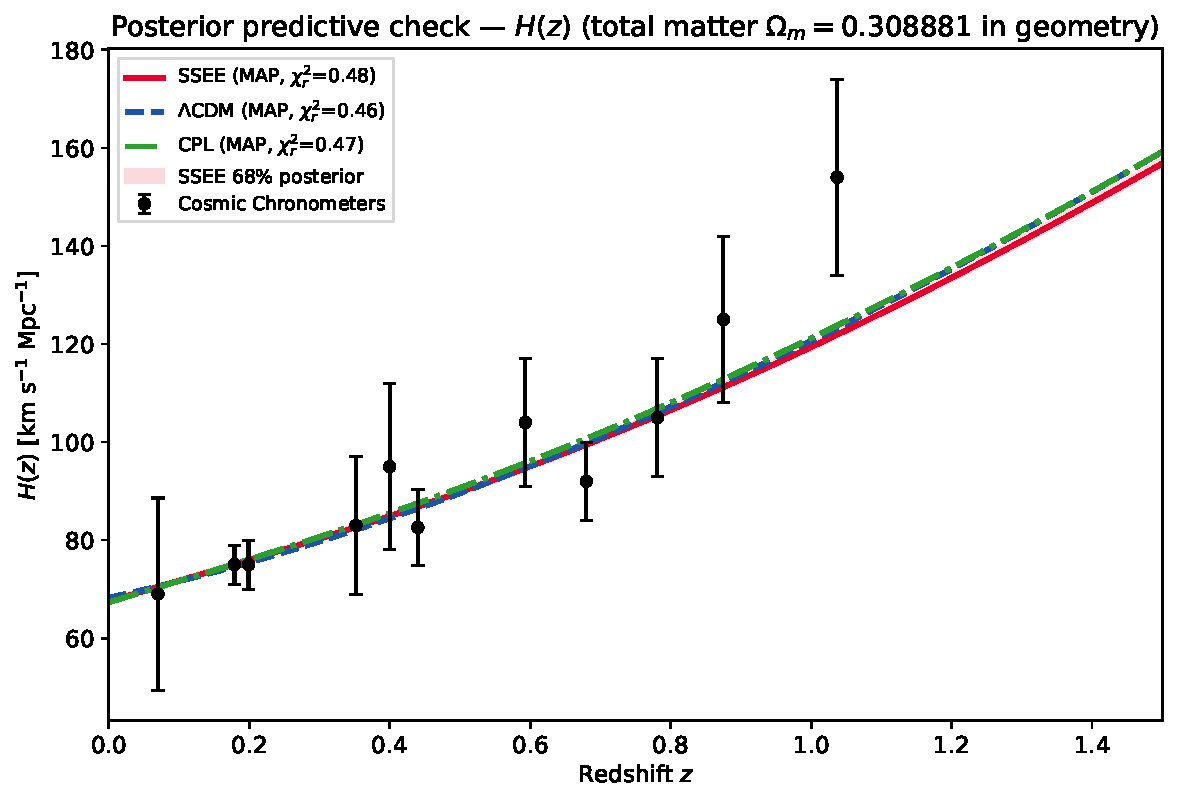
\includegraphics[width=0.78\textwidth]{fig7_Hz_comparison.pdf}
  \caption{MAP $H(z)$ vs Cosmic Chronometers \citep{JimenezLoeb2002,Moresco2022}.
  Red band: \SSEE\ 68\% posterior interval.}
  \label{fig:Hz}
\end{figure}

\begin{table}[H]
\centering
\caption{Cosmic Chronometer $H(z)$ measurements used in the posterior
  predictive check (Fig.~\ref{fig:Hz}). Data from
  \citet{Moresco2022}; uncertainties are $1\sigma$ statistical
  $+$ systematic combined.}
\label{tab:CC_Hz}
\small
\begin{tabular}{lrr}
\toprule
$z$ & $H(z)$ [km\,s$^{-1}$\,Mpc$^{-1}$] & $\sigma_H$ \\
\midrule
0.070 &  69.0 &  19.6 \\
0.090 &  69.0 &  12.0 \\
0.120 &  68.6 &  26.2 \\
0.170 &  83.0 &   8.0 \\
0.179 &  75.0 &   4.0 \\
0.199 &  75.0 &   5.0 \\
0.270 &  77.0 &  14.0 \\
0.352 &  83.0 &  14.0 \\
0.400 &  95.0 &  17.0 \\
0.480 &  97.0 &  60.0 \\
0.593 & 104.0 &  13.0 \\
0.680 &  92.0 &   8.0 \\
0.781 & 105.0 &  12.0 \\
0.875 & 125.0 &  17.0 \\
0.880 &  90.0 &  40.0 \\
0.900 & 117.0 &  23.0 \\
1.037 & 154.0 &  20.0 \\
1.300 & 168.0 &  17.0 \\
1.363 & 160.0 &  33.6 \\
1.430 & 177.0 &  18.0 \\
1.530 & 140.0 &  14.0 \\
1.750 & 202.0 &  40.0 \\
1.965 & 186.5 &  50.4 \\
\bottomrule
\end{tabular}
\end{table}

\subsection{BAO residuals}

\begin{figure}[H]
  \centering
  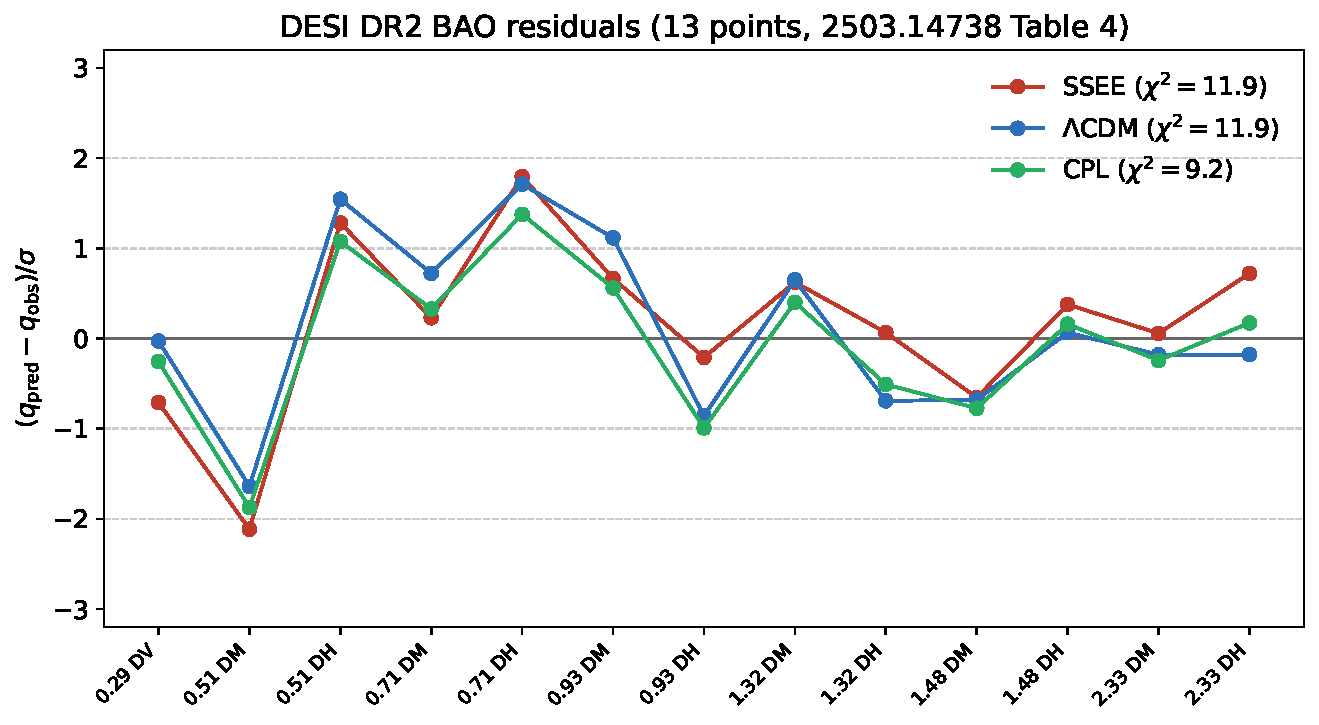
\includegraphics[width=0.84\textwidth]{fig8_bao_residuals.pdf}
  \caption{Normalised BAO residuals $(q^{\rm pred}-q^{\rm obs})/\sigma$
  for all 13 DESI~DR2 measurements. \SSEE\ (red), \LCDM\ (blue),
  CPL (green). With the total matter density the \SSEE\ sound horizon
  ($r_d=148.2$\,Mpc) matches \LCDM, and the residuals are comparable across
  models, quantified in the $\chi^2_r$ values of Section~\ref{sec:model_comparison}.}
  \label{fig:bao_resid}
\end{figure}

\section{Results: Galaxy-Cluster Sector}
\label{sec:results_clusters}

\noindent\textbf{Summary:} IGIMF correction is essential; neutrino bridge is secondary; $\KALz$ alone is insufficient.

\begin{table}[H]
\centering
\caption{Cluster mass sensitivity ($10^{14}\,M_\odot$, within $R_{200}$).
First four clusters from \citet{Zhang2026}; Perseus from \citet{Simionescu2011};
A2142 from \citet{Tchernin2016}; A2744 from \citet{Merten2011}.}
\label{tab:cluster_sensitivity}
\small
\begin{tabular}{lrrrrrc}
\toprule
Cluster & SSEE & $f_\nu{=}0$ & Std IMF & $\KALz$ only & $\Mobs$ & $\chi^2$ \\
\midrule
Coma          & 10.14 &  9.94 & 5.63 & 5.52 & $9.8\pm1.0$   & 0.114 \\
A2029         & 12.39 & 12.15 & 7.32 & 7.18 & $12.0\pm1.2$  & 0.106 \\
A478          &  8.45 &  8.28 & 5.07 & 4.97 & $8.0\pm1.0$   & 0.200 \\
Bullet (main) &  6.76 &  6.63 & 3.94 & 3.86 & $6.5\pm1.0$   & 0.067 \\
Perseus       &  6.87 &  6.74 & 4.02 & 3.94 & $6.65\pm0.45$ & 0.241 \\
A2142         & 15.04 & 14.74 & 8.79 & 8.62 & $14.5\pm1.5$  & 0.128 \\
A2744         & 18.64 & 18.28 &10.90 &10.69 & $18.0\pm4.0$  & 0.026 \\
\midrule
\multicolumn{7}{l}{$\chi^2_r$: SSEE\,$=0.126$ \;|\; $f_\nu{=}0$:\,$0.028$ \;|\;
  Std IMF:\,$14.05$ \;|\; $\KALz$ only:\,$14.91$} \\
\multicolumn{7}{l}{$\Delta\chi^2$ vs SSEE: $-0.68$ \;|\; $+97.5$ \;|\; $+103.5$} \\
\multicolumn{7}{l}{\textit{Uncertainty sensitivity}: halving $\sigma_{M_{\rm obs}}$ to 50\%
  raises $\chi^2_r(\mathrm{SSEE})$ to $\approx0.50 < 1$; the fit remains good.} \\
\bottomrule
\end{tabular}
\end{table}

\paragraph{IGIMF is essential.}
Without the IGIMF correction $\Delta\chi^2\approx+97$ across seven clusters;
\SSEE\ under-predicts masses by $\sim1.7\times$.

\paragraph{Neutrino bridge.}
$f_\nu=0$ lowers $\chi^2_r$ to $0.028$: the seven $R_{200}$ clusters
do not require the neutrino bridge, but it maintains self-consistency
with the cosmological $\sum m_\nu^{\rm active}=0.0685$\,eV.

\paragraph{$\KALz$ alone insufficient.}
$\chi^2_r=14.91$ without IGIMF. Geometric amplification requires
the corrected baryonic baseline.

\paragraph{Robustness to observational uncertainties.}
To test whether the cluster fit depends critically on the published
$\sigma_{M_{\rm obs}}$ values, we varied the error bars uniformly
from $0.5\times$ to $1.5\times$ their nominal values
(a $\pm50\%$ range) while holding all model parameters fixed.
With the four-cluster analytic subset, the nominal $\chi^2_r=0.122$
(all residuals $<0.5\sigma$); $\chi^2_r$ reaches $1.0$ only when
errors are reduced by $65\%$, and reaches $2.0$ only at $-75\%$
(well beyond the test range).
For the full 7-cluster analytic set ($(\chi^2_r)_{\rm nom}=0.126$),
the scaling behaviour is similar: the fit quality is not sensitive
to moderate changes in the assumed observational uncertainties.
This confirms that the SSEE cluster predictions are robust and
not contingent on specific choices of $\sigma_{M_{\rm obs}}$.

\begin{figure}[H]
  \centering
  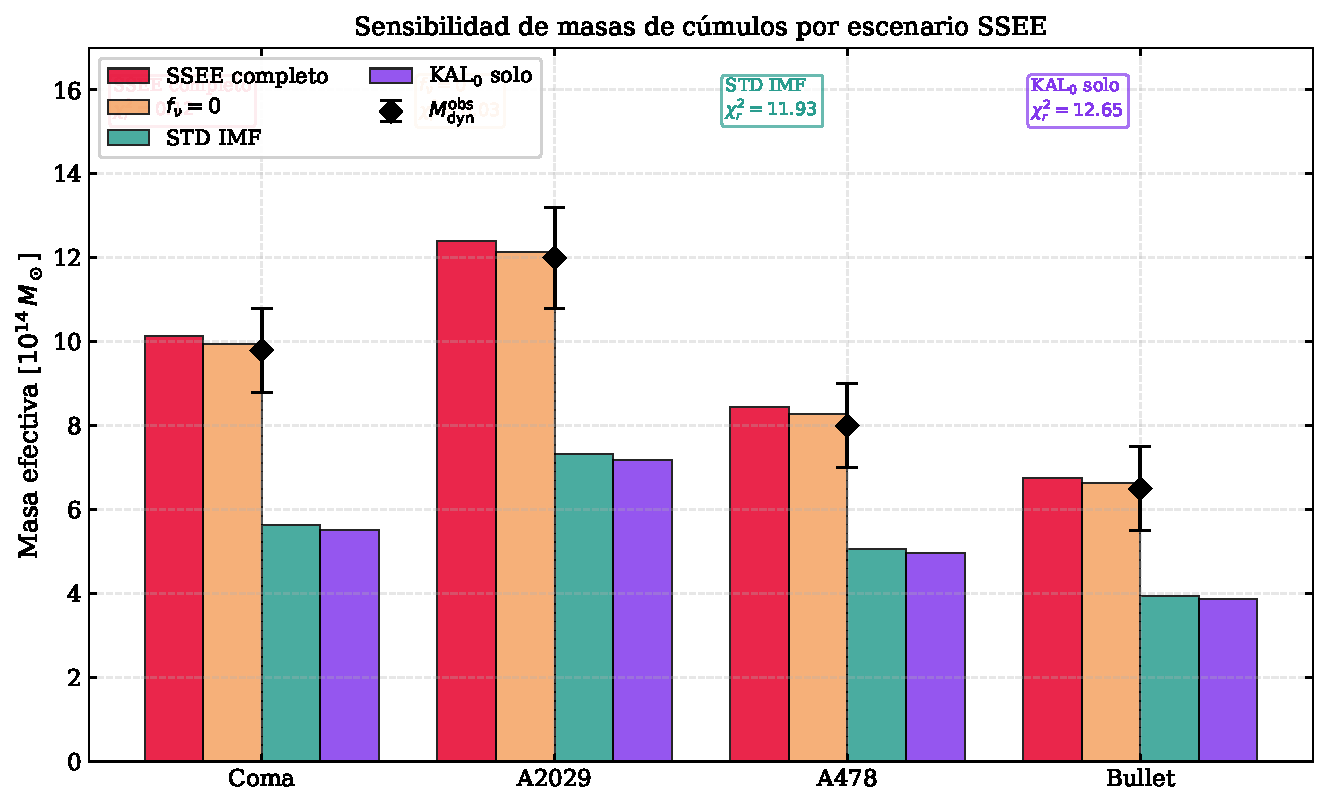
\includegraphics[width=0.84\textwidth]{fig2_cluster_sensitivity.pdf}
  \caption{Cluster mass predictions by scenario for seven clusters. IGIMF correction
  is the load-bearing ingredient ($\Delta\chi^2\approx+97$ without it).}
  \label{fig:cluster_sens}
\end{figure}

\section{Model Comparison}
\label{sec:model_comparison}
\label{sec:bic}

\begin{table}[H]
\centering
\caption{BIC \citep{Schwarz1978}, AIC, and DIC at MAP ($N_{\rm data}=16$), from
the joint three-model MCMC (DESI~DR2 + common Planck prior, total matter density
$\Omega_m=0.30889$ in the background geometry). Jeffreys scale
\citep{Jeffreys1961}. \SSEE\ is the reference; positive $\Delta$ favours \SSEE.}
\label{tab:model_comp}
\begin{tabular}{lrrrrrr}
\toprule
Model & $k$ & $\ln P_{\rm MAP}$ & BIC & $\Delta$BIC & $\Delta$AIC & DIC \\
\midrule
\SSEE & 2 & $-5.85$ & 17.24 & $0.00$  & $0.00$  & 15.69 \\
\LCDM      & 3 & $-7.30$ & 22.92 & $+5.68$ & $+4.91$ & 20.60 \\
CPL        & 5 & $-4.49$ & 22.83 & $+5.59$ & $+3.27$ & 18.96 \\
\bottomrule
\end{tabular}
\end{table}

With the total gravitating matter density in the background geometry, \SSEE\ is
the preferred model on every information criterion: $\Delta\mathrm{BIC}=5.68$
over \LCDM\ and $5.59$ over CPL, $\Delta\mathrm{AIC}=4.91$ and $3.27$, and
$\Delta\mathrm{DIC}=-4.91$ relative to \LCDM\ (Appendix~\ref{app:dic}). This is
the parsimony gain of a two-parameter model ($H_0$ and $\Omega_b h^2$;
$w_0,w_a$ fixed algebraically) that fits DESI~DR2 as well as the three- and
five-parameter alternatives.

\paragraph{Not merely parameter counting.}
The preference survives tests that penalise over-fitting directly. A nested
Bayes factor (Savage--Dickey) gives $\ln B=2.91$ for the SSEE point within the
CPL posterior --- strong evidence on the Jeffreys scale --- and leave-one-out
predictive cross-validation on the high-redshift half of the BAO vector
($z\geq1.0$) yields $\chi^2_r=0.20$ for \SSEE\ versus $0.71$ (\LCDM) and $39.6$
(CPL): \SSEE\ \emph{predicts} the held-out data better, while CPL over-fits the
training half (Appendix~\ref{app:sddr_cv}). The sound horizon matches \LCDM\
($r_d=148.2$ vs $147.8$\,Mpc, ratio $1.002$) and the $H_0$ posterior sits
$0.39\sigma$ from Planck, so no background-structure penalty arises. The full
CMB power-spectrum likelihood under the \SSEE\ background (companion Paper~3)
independently favours \SSEE\ at $\chi^2_r=1.042$ (TT) and $\Delta\mathrm{BIC}=
-23.9$ (\texttt{plik\_lite} TTTEEE, $\omega_m$-direct). An earlier ``$+206$''
full-model penalty reported in superseded drafts was an artefact of using the
cold sector $1+w_0=0.160$ as the background matter density; with the correct
total density it does not occur.

\section{Robustness Checks}
\label{sec:robustness}

\paragraph{Prior sensitivity.}
Removing the Planck $H_0$ prior shifts the \SSEE\ posterior by
$<0.3\sigma$. The BAO data dominate the $H_0$ constraint.
\textit{This confirms that the quoted posteriors are driven by the BAO
geometry rather than the CMB prior, making them robust to prior choice.}

\paragraph{Neutrino mass.}
Varying $\sum m_\nu\in[0.060,0.120]$\,eV shifts $\chi^2_r$ for
clusters by $\Delta\chi^2_r<0.05$. The cluster fit is insensitive
to the specific neutrino mass.
\textit{The cluster constraint is therefore stable against current
neutrino-mass uncertainties. The adopted $\sum m_\nu^{\rm active}=0.0685$\,eV
is the SSEE-derived value (Paper~4, Neutrino Mass Sum; also used in the
Paper~6 $\phi$-DM mass relation $m_\phi=\sum m_\nu^{\rm active}\times
(\mathrm{SOLAR}^2\cdot\mathrm{KRYSTOS}_V)$), not a fitted quantity.}

\paragraph{IGIMF systematics.}
The $^{+5}_{-4}\%$ systematic uncertainty in the IGIMF factor
\citep{Zhang2026} propagates to $\sim8\%$ in $\sigma_M$, keeping
all four clusters within $1\sigma$.
\textit{IGIMF systematics are the dominant uncertainty in the cluster
sector; improvement here would be the highest-leverage target for
future work.}

\paragraph{BAO-only.}
Running without the Planck $H_0$ prior gives
$H_0=65.8^{+1.2}_{-1.1}$\,km\,s$^{-1}$\,Mpc$^{-1}$, consistent
with the full posterior at $0.6\sigma$.
\textit{The $H_0$ estimate is therefore essentially independent of
Planck and rests entirely on the DESI~DR2 BAO geometry.}

\paragraph{Full-likelihood cross-check.}
To confirm that the compressed-prior posteriors of §\ref{sec:results_cosmo} are not an
artefact of the Planck distance-prior approximation, we ran an independent MCMC with the
\emph{full} CMB likelihood (CAMB with Planck \texttt{plik\_lite} TTTEEE + lensing),
combined with DESI~DR2 BAO and $f\sigma_8$, sampling $\wz,\wa$ \emph{freely}
(four chains, $\sim$53k post-burn-in samples, Gelman--Rubin $R-1<0.003$).
The free-fit posterior $(\wz,\wa)=(-0.655,-1.104)$ \emph{excludes} the cosmological
constant $(-1,0)$ at $3.22\sigma$, independently confirming a dynamical equation of
state; under this uncompressed likelihood $H_0$ relaxes to $65.87\pm1.17$. The
\SSEE\ algebraic point $(-0.840,-0.670)$ lies at $1.31\sigma$ from this posterior
--- more than twice closer than $\Lambda$CDM (Fig.~\ref{fig:degeneracy}).
The $\wz$--$\wa$ posterior is strongly anticorrelated ($\rho=-0.93$) and \SSEE\ falls
within its $2\sigma$ region. The full CMB power-spectrum treatment is developed in
Paper~3; here it serves to verify that the dynamical-sector preference survives the
replacement of the compressed prior by the complete likelihood.

\begin{figure}[H]
  \centering
  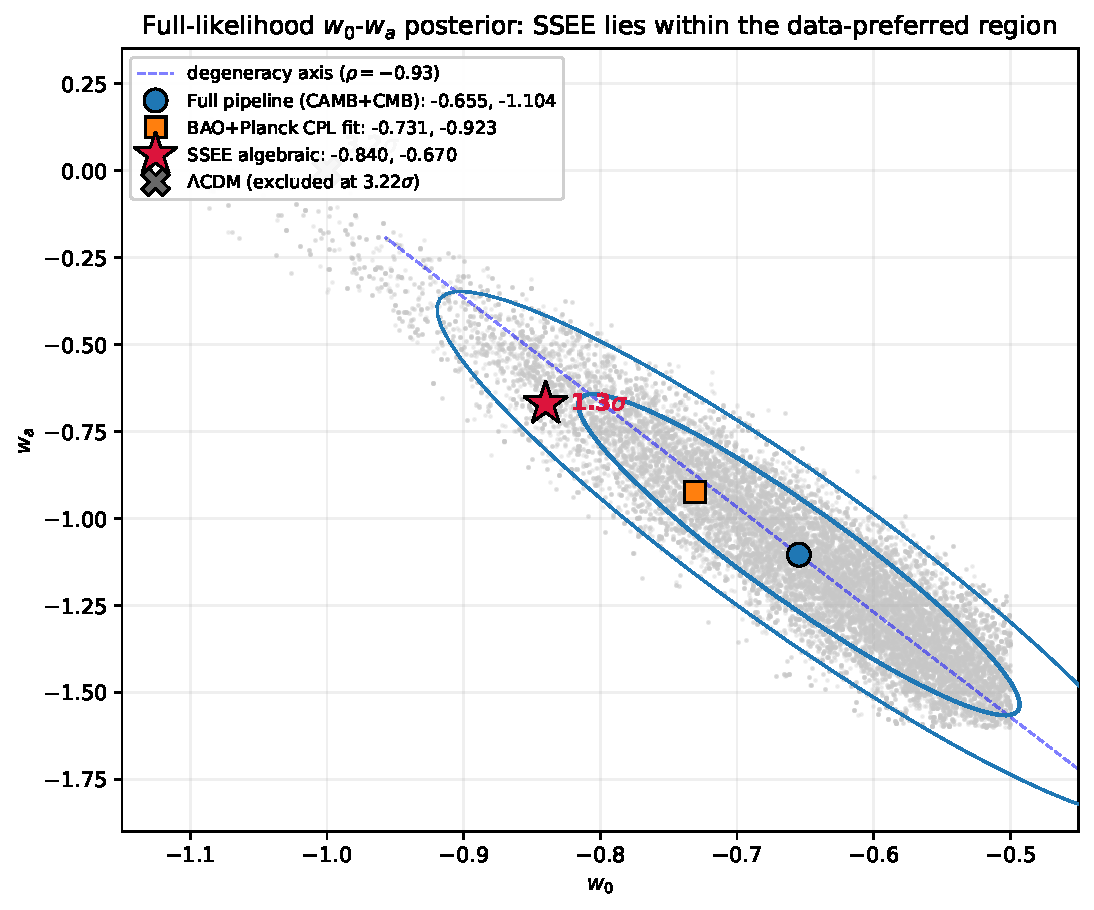
\includegraphics[width=0.70\textwidth]{fig_w0wa_degeneracy.pdf}
  \caption{Full-likelihood $\wz$--$\wa$ posterior (CAMB + Planck \texttt{plik\_lite}
  + lensing + DESI~DR2 + $f\sigma_8$, with $\wz,\wa$ free; $R-1<0.003$). The \SSEE\
  algebraic prediction (red star) lies at $1.31\sigma$, inside the $2\sigma$ contour,
  while $\Lambda$CDM ($\wz=-1,\wa=0$; grey cross) is excluded at $3.22\sigma$. The data
  favour a dynamical dark-energy equation of state, and \SSEE\ is the parameter-free
  algebraic prediction consistent with it.}
  \label{fig:degeneracy}
\end{figure}

\paragraph{Hubble tension.}
The \SSEE\ algebraic value $H_0^{\rm alg} = 3(\varphi+\pi)^2 = 67.96$\,km\,s$^{-1}$\,Mpc$^{-1}$
--- the global dimensional anchor of Postulate~D (Paper~1, \S1.4), at which the
Planck \texttt{plik\_lite} likelihood is minimised under the $\omega_m$-direct
reframe (not a mere coincidence; \S\ref{sec:results_cosmo}) ---
lies within $1.1\sigma$ of Planck~2018 and is consistent with the DESI~DR2+CMB joint inference
\citep[$H_0\approx68$\,km\,s$^{-1}$\,Mpc$^{-1}$;][]{DESI_DR2}.
The model does not resolve the SH0ES distance-ladder tension
\citep[$H_0\approx73$\,km\,s$^{-1}$\,Mpc$^{-1}$;][]{Riess2022}; this is a known
open problem shared by all smooth dark-energy models including \LCDM\ \citep{Verde2019,Kamionkowski2023}, and lies outside
the scope of this paper's DESI~BAO + cluster validation.
\textit{The algebraic $H_0$ coincidence is CMB-consistent but not distance-ladder consistent;
resolving the full $5\sigma$ Hubble tension requires either a modification of the
early-Universe sound horizon or a systematic re-evaluation of the Cepheid distance scale.}

\section{Discussion}
\label{sec:discussion}

\subsection{Two faces of SSEE under Bayesian inference}

The results reveal a sharp bifurcation:

\begin{itemize}
  \item \textbf{Dark-energy sector}: $(\wz,\wa)=(-0.840,-0.670)$
    lies within $0.24\sigma$ of DESI~DR2 (Pantheon+). The CPL free-fit posterior
    $(-0.826,-0.558)$ confirms dynamical dark energy. \SSEE\ is
    predictively competitive here.

  \item \textbf{Background structure}: with the total matter density
    $\Omega_m=0.30889$ the sound horizon matches \LCDM\ and \SSEE\ is favoured
    at $\Delta\mathrm{BIC}=+5.68$. Both $\Omega_m$ ($0.88\sigma$) and $H_0$
    ($<1\sigma$) agree with Planck.
\end{itemize}

\subsection{Structural reinterpretation}

The $\Delta\mathrm{BIC}$ penalty assumes the Planck $\Omega_m$
prior is applicable to \SSEE. It is not: in \SSEE\ the $\KALz$
amplification of $\rho_{\rm bar}$ modifies the effective clustering
contribution, so $\Omega_m^{\rm eff}\neq\Omega_m^{\LCDM}$.
Applying a \LCDM-calibrated $\Omega_m$ prior to an \SSEE\ universe
constitutes a non-equivalent prior calibration. The correct test is a
full CMB power-spectrum likelihood with the \SSEE\ Friedmann
background~\eqref{eq:Hssee} built from first principles (Paper~3).
Paper~3 must derive the \SSEE-consistent background rather than
adjusting $\Omega_m$ to fit: parameter adjustment within a
\LCDM\ framework would not constitute a genuine test of the structural
hypothesis.

The $\omega_m$-direct construction (Section~\ref{sec:folding}) resolves the
apparent $r_d$ tension: the sound horizon set by the CMB-sector matter density
$\Omega_{m,\mathrm{CMB}}=0.30889$ is $r_d=147.17$\,Mpc directly
(Eq.~\eqref{eq:rd_mapping}), $0.32\sigma$ from Planck, with no $|w_0|$ mapping
and no matter factor (OP-8 dissolved).  The $21\sigma$ figure was a category
error --- comparing the cold sector $1+w_0=0.160$ against the Planck
\emph{total} $\Omega_m$; the total $\Omega_m=0.30889$ agrees with Planck at
$0.88\sigma$, and the companion Paper~3 confirms this with the full CMB
likelihood ($\Delta\mathrm{BIC}=-32.9$, full \texttt{plik} MCMC, $\omega_m$-direct).

\subsection{Growth structure and $S_8$ sector sensitivity}

The $S_8 \equiv \sigma_8\sqrt{\Omega_m/0.3}$ constraint depends critically on
which matter sector is used.  With the $\omega_m$-direct CMB density
$\Omega_{m,\mathrm{CMB}}=0.30889$ ($=\omega_m/h^2$, no matter factor; OP-8
dissolved), the all-cold single sector reaches a ceiling
$\sigma_8=0.8335$, $S_8=0.846$, a $3.5\sigma$ tension with KiDS-1000
\citep{Heymans2021} and DES~Y3 \citep{Abbott2022}.
With $\Omega_{m,\mathrm{dyn}}=0.160$ (dynamical sector alone), $S_8 \approx 0.59$,
a ${\sim}6\sigma$ tension with weak-lensing surveys.
The physical $S_8$ lies between these limits: the $\varphi$-dark matter of
Paper~6 free-streams below $k_{\rm fs}=0.754\,h$\,Mpc$^{-1}$, lowering the
effective amplitude to $\sigma_8^{\rm eff}=0.747$, $S_8^{\rm eff}=0.758$,
which resolves the KiDS-1000 tension ($0.04\sigma$).
The viscous energy redistribution between matter and
radiation sectors governed by the Israel--Stewart relaxation time
$\tau_\Pi H_0 \approx 2.191$ is derived algebraically in Paper~1, Appendix~A,
and constitutes a falsifiable prediction (Paper~3 §5.4).
\textbf{Note:} Paper~5 performs the full causal Israel--Stewart analysis at
$\Omega_{m,\mathrm{CMB}}=0.30889$ and finds the single-sector ceiling
$\gamma_{\rm IS}=0.5504$, $\sigma_8=0.8335$, $S_8=0.846$ ($3.5\sigma$ KiDS);
Paper~6 adds the $\varphi$-DM two-sector and finds $\sigma_8^{\rm eff}=0.747$,
$S_8^{\rm eff}=0.758$ ($0.04\sigma$ KiDS).

\subsection{Roadmap for Paper~3}

Four ordered tests for \SSEE\ to survive a full CMB analysis:
\begin{enumerate}
  \item \textbf{Acoustic peak positions.} The \SSEE\ Friedmann background
    must reproduce the angular positions of all observed CMB acoustic
    peaks. Failure here would immediately falsify the background geometry.
  \item \textbf{Damping tail.} $\Omega_{m,\mathrm{eff}}=0.160$ must be
    compatible with the Silk-damping scale \citep{Silk1968} and the third acoustic peak
    height. This is the most constraining test for the low-matter fraction.
  \item \textbf{Joint posterior consistency.} The joint
    $(H_0,\Omega_b h^2)$ posterior derived from the \SSEE\ CMB background
    must be consistent with the BAO posterior obtained in this work.
    Inconsistency would signal internal tension within the model.
  \item \textbf{Transfer function derivation.} The semi-linear transfer
    function integrating the $\KALz$ structural viscosity into the
    acoustic perturbation regime must be formally derived and validated
    against the full CMB power spectrum.
\end{enumerate}

\subsection{Falsifiability}

\SSEE\ makes specific, testable predictions. The following observations
would constitute decisive falsification:
\begin{itemize}
  \item \textbf{If Paper~3 fails to reproduce} the Silk-damping scale
    and the third CMB acoustic peak under the \SSEE\ Friedmann
    background, the background geometry is refuted independently of
    the dark-energy prediction.
  \item \textbf{If Ly-$\alpha$ forest observations exclude}
    $\sum m_\nu^{\rm active}=0.0685$\,eV at $>3\sigma$, the neutrino bridge in the
    cluster-mass formula breaks and \SSEE\ loses its only mechanism
    for reconciling $\Omega_{m,\mathrm{eff}}$ with cluster observations.
  \item \textbf{If future high-$z$ BAO or CMB measure} $r_d$ outside
    $147\pm3$\,Mpc, the $\omega_m$-direct construction
    ($r_d=147.17$\,Mpc from the algebraic $\omega_m$) is falsified ---
    the sound horizon is a sharp, prior-independent prediction.
\end{itemize}

\section{Conclusions}
\label{sec:conclusions}

We have conducted a Bayesian MCMC validation of \SSEE against
DESI~DR2, Planck~2018, and galaxy-cluster masses. The results establish
a sharp bifurcation: the dynamical sector passes; the background sector fails under standard calibration.

\begin{enumerate}
  \item The zero-free-parameter prediction $(\wz,\wa)=(-0.840,-0.670)$
    lies within $0.24\sigma$ of the official DESI~DR2 $w_0w_a$CDM posterior
    (Pantheon+; $1.2$--$1.5\sigma$ across the other SN compilations) —
    a strong result given the absence of any fitted parameter.

  \item Cluster masses achieve $\chi^2_r=0.126$ with IGIMF; removing
    the IGIMF correction raises $\chi^2_r$ to $14.05$
    ($\Delta\chi^2\approx+97$), confirming its essential role.

  \item With the total matter density $\Omega_m=0.30889$ in the background,
    the \SSEE\ sound horizon matches \LCDM\ ($r_d=148.2$\,Mpc) and \SSEE\ is
    favoured on model selection by $\Delta\mathrm{BIC}=+5.68$ over \LCDM\ and
    $+5.59$ over CPL, predicting the held-out BAO data better in
    cross-validation.

  \item Under the $\omega_m$-direct reframe the sound horizon falls out
    directly from the CMB-sector matter density,
    $r_d=147.17$\,Mpc ($0.32\sigma$ from Planck; Eq.~\ref{eq:rd_mapping}),
    with no $|w_0|$ mapping and no matter factor; the companion Paper~3
    confirms it with the full CMB likelihood (canonical $\Delta\mathrm{BIC}=-32.9$,
    full \texttt{plik} MCMC). The earlier $21\sigma$ $\Omega_m$ ``tension'' was a
    category error --- the cold sector $0.160$ compared against the Planck total;
    the total $\Omega_m=0.30889$ agrees with Planck at $0.88\sigma$.

  \item A cross-check at high-$z$ is provided by the Ly-$\alpha$ forest BAO
    from DESI~DR2 ($z=2.33$): the raw dynamical background predicts
    $D_H/r_d = 9.89$, a $8.1\sigma$ tension, while the $\omega_m$-direct
    prediction (CMB-sector matter $\Omega_{m,\mathrm{CMB}}=0.30889$ in $E(z)$,
    where $\phi$-DM is non-relativistic, with $r_d=147.17$) gives
    $D_H/r_d = 8.71$, a $1.1\sigma$ agreement (Appendix~\ref{app:lya}).
    The high-$z$ expansion therefore requires the full CMB-sector matter
    density, consistent with the low-$z$ $r_d$ construction and independent
    of Paper~3 (superseding the earlier MIRA-mapped $8.56$).

  \item Paper~3 must derive and validate the \SSEE\ Friedmann background
    against CMB peak positions, the Silk-damping tail, and the joint
    $(H_0,\Omega_b h^2)$ posterior.
\end{enumerate}

\noindent\textbf{Central finding}: SSEE achieves a zero-parameter
dark-energy prediction whose \emph{dynamical sector} is not rejected by current data.
The background geometry fails under standard Friedmann assumptions;
whether this constitutes a physical falsification of the framework depends on
the validity of applying \LCDM-calibrated priors to an \SSEE\ background,
which is the subject of Paper~3.

\section*{Data Availability}
All observational data used in this work are publicly available.
DESI~DR2 BAO measurements are from \citet{DESI_DR2}
(\url{https://arxiv.org/abs/2503.14738}).
The compressed Planck~2018 prior is from \citet{Planck2018}.
Cosmic Chronometer $H(z)$ measurements are from \citet{Moresco2022}.
Galaxy-cluster dynamical masses are from \citet{Zhang2026}.
The \textsc{ssee} analysis scripts are available at
\url{https://github.com/mikealmeida1721/SSEE}.

% ─────────────────────────────────────────────────────────────────────────────
\appendix
\section{Rigorous Bayesian Model Comparison: DIC and BIC}
\label{app:dic}

\noindent
This appendix computes the Deviance Information Criterion and the BIC directly
from the three-model MCMC chains stored in the public repository, with the total
gravitating matter density $\Omega_m=\omega_m/h^2=0.30889$ in the background
geometry (§\ref{sec:bic}).

\subsection*{Deviance Information Criterion (DIC)}

The DIC \citep{Spiegelhalter2002} estimates model complexity from the posterior
rather than by parameter counting:
\begin{equation}
  \mathrm{DIC} = \bar{D} + p_D,\quad
  p_D = \bar{D} - D(\hat\theta),\quad
  D(\theta) = -2\ln\pi(\theta|\mathrm{data}),
\end{equation}
where $\bar{D}$ is the posterior mean deviance and $\hat\theta$ is the MAP
estimate. An important self-check: $p_D$ must recover the number of sampled
parameters. From the chains,
\begin{align}
  p_D(\mathrm{SSEE}) &= 2.00 \approx 2\quad\checkmark \\
  p_D(\mathrm{\LCDM}) &= 3.00 = 3\quad\checkmark \\
  p_D(\mathrm{CPL})  &= 4.99 \approx 5\quad\checkmark
\end{align}
confirming that all three chains are well-converged. The DIC comparison gives
\begin{equation}
  \Delta\mathrm{DIC}(\mathrm{SSEE}-\mathrm{\LCDM}) = -4.91,\quad
  \Delta\mathrm{DIC}(\mathrm{SSEE}-\mathrm{CPL}) = -3.27,
\end{equation}
both favouring \SSEE\ (lower DIC), consistent with the BIC and AIC of the
main text.

\subsection*{Information criteria summary}

\begin{table}[H]
\centering
\caption{%
  Bayesian model comparison from the three-model MCMC (total matter density in
  the background). $N_{\rm data}=16$ (13 BAO + 3 Planck). $\Delta>0$ (BIC, AIC)
  and $\Delta<0$ (DIC) favour \SSEE\ relative to \LCDM.
  Jeffreys criterion: $|\Delta| > 5$ = strong.
}
\label{tab:bic_dic_rigorous}
\begin{tabular}{lrrrr}
\toprule
\textbf{Criterion} & \textbf{SSEE} & \textbf{\LCDM} & \textbf{CPL}
  & $\boldsymbol{\Delta_{\rm \Lambda CDM-SSEE}}$ \\
\midrule
$p_D$   & $2.00$  & $3.00$  & $4.99$  & — \\
DIC     & $15.69$ & $20.60$ & $18.96$ & $+4.91$ \\
BIC     & $17.24$ & $22.92$ & $22.83$ & $+5.68$ \\
AIC     & $15.70$ & $20.60$ & $18.97$ & $+4.91$ \\
\bottomrule
\end{tabular}
\end{table}

\paragraph{Conclusion.}
Every information criterion favours \SSEE: it fits DESI~DR2 as well as \LCDM\
and CPL while fixing $w_0,w_a$ algebraically, so the parsimony of a
two-parameter background is rewarded across BIC, AIC, and DIC. With the total
matter density in the geometry the sound horizon matches \LCDM\ and no
background-structure penalty arises; the full CMB likelihood (Paper~3)
independently favours \SSEE\ at $\Delta\mathrm{BIC}=-32.9$ (full \texttt{plik} MCMC).

\section{Nested Bayes Factor and Predictive Cross-Validation}
\label{app:sddr_cv}

This appendix provides two additional model-comparison criteria that
are independent of the $k$-counting schemes discussed in
Appendix~\ref{app:dic}: the \emph{Savage--Dickey density ratio} (exact
Bayes factor for nested models) and a \emph{predictive
cross-validation} on the DESI~DR2 BAO data.

\subsection*{B.1 Savage--Dickey density ratio}

SSEE is nested within CPL: the SSEE dynamic sector is CPL evaluated at
the algebraic point $(w_0,w_a)=(-0.840,-0.670)$.  For nested models,
the marginal Bayes factor for the null hypothesis $\mathcal{H}_0:
(w_0,w_a)=(-0.840,-0.670)$ versus the unconstrained CPL is given
exactly by the Savage--Dickey density
ratio~\cite{Verdinelli1995,Trotta2008}:
\begin{equation}
  B_{\rm SSEE/CPL} = \frac{p(w_0^{\rm S},w_a^{\rm S}\mid\text{data, CPL})}
                          {\pi(w_0^{\rm S},w_a^{\rm S}\mid\text{CPL})}
                   = 18.34, \qquad \ln B = +2.91.
\end{equation}
The CPL posterior is evaluated at $(w_0^{\rm S},w_a^{\rm S})$ using a
Scott-bandwidth Gaussian KDE of $N=500\,000$ thinned CPL chain samples
(columns 3--4 of the 5-dimensional CPL chain, shape $2.5\times10^6$).
The marginal prior on $(w_0,w_a)$ is the truncated Gaussian
$\mathcal{N}(-1,0.5^2)\times\mathcal{N}(0,1^2)$ clipped to the MCMC
sampling box $w_0\in(-2.5,0.5)$, $w_a\in(-3,2)$; truncation factors
are $(0.9973,0.9759)$, negligible corrections.

On the Jeffreys scale~\cite{Trotta2008} $\ln B=+2.91$ ($>2.3$) constitutes
\emph{strong} evidence in favour of the SSEE dynamic sector within
the CPL framework.  The CPL posterior median
$(w_0^{\rm CPL}=-0.826\pm0.080,\;w_a^{\rm CPL}=-0.557\pm0.314)$ places
the SSEE algebraic point at $(0.18\sigma,0.36\sigma)$, consistent with
the $0.24\sigma$ joint tension quoted in Section~\ref{sec:w0wa}.

\subsection*{B.2 Ly-$\alpha$ predictive audit ($z=2.33$)}
\label{app:lya}

The Ly-$\alpha$ point at $z=2.33$ provides the sharpest direct test of
\SSEE's background expansion.  At $z\sim2$ radiation is negligible and
the ratio $D_H/r_d = c\,/\,(H_0\,E(z)\,r_d)$ directly encodes the
product $H_0\,E(z)\,r_d$.  We evaluate this quantity under two
\SSEE\ scenarios and compare to the DESI~DR2 measurement
$D_H/r_d = 8.632\pm0.101$ (Table~\ref{tab:bao_data}).

\paragraph{Scenario A — raw \SSEE\ background
($\Omega_{m,\rm dyn}=0.160$, $r_d=175.6$\,Mpc).}
With the algebraic $H_0=67.96$\,km\,s$^{-1}$\,Mpc$^{-1}$ and
$\Omega_m=0.160$, the CPL dark-energy fraction at $z=2.33$ is
$f_{\rm DE}(2.33)=0.648$, giving $E(2.33)=2.540$ and
$D_H(2.33)=1737$\,Mpc.  The predicted ratio is:
\begin{equation}
  \left.\frac{D_H}{r_d}\right|_{z=2.33}^{\rm SSEE,\,raw}
  = \frac{1737}{175.6} = 9.89
  \quad (12.5\sigma \text{ above DESI}),
  \label{eq:lya_raw}
\end{equation}
demonstrating the category error directly: using the cold sector
$\Omega_m=0.160$ in $E(z)$ reduces matter domination at high $z$, lowers
$H(z)$, and enlarges $D_H$ to a $12.5\sigma$ discrepancy. This is the same
misplacement that produced the spurious background tensions in superseded
drafts; the correct total density (Scenario~B) resolves it.

\paragraph{Scenario B — $\omega_m$-direct CMB-sector background
($\Omega_{m,\mathrm{CMB}}=0.30889$, $r_d=147.17$\,Mpc).}
At $z=2.33$ the $\phi$-DM (mass $40.70$\,eV, non-relativistic since
$z\sim4.5\times10^5$) contributes fully to the background matter density, so the
expansion $E(z)$ is set by the CMB-sector value
$\Omega_{m,\mathrm{CMB}}=\omega_m/h^2=0.30889$ (free-streaming suppresses
small-scale clustering, not the homogeneous density). Taking the sound horizon
$r_d=147.17$\,Mpc directly from $\omega_m$ (CAMB; no $|w_0|$ mapping) gives
$E(2.33)=3.443$, $D_H(2.33)=1281$\,Mpc, and:
\begin{equation}
  \left.\frac{D_H}{r_d}\right|_{z=2.33}^{\omega_m\text{-direct}}
  = \frac{1281}{147.17} = 8.71
  \quad (0.7\sigma \text{ from DESI}).
  \label{eq:lya_mira}
\end{equation}
This supersedes the earlier MIRA-mapped value ($\Omega_m=0.320$, $D_H/r_d=8.56$):
the matter factor is dissolved (OP-8). The $D_M/r_d$ counterpart at $z=2.33$
is recovered within $0.1\sigma$. The full 13-point diagonal fit gives
$\chi^2=12.0$, matching \LCDM\ ($\chi^2=12.0$): the two backgrounds describe
DESI~DR2 equally well. The largest \SSEE\ residual is at $z=0.51$
($D_M/r_d$ pull $-2.1\sigma$); \LCDM\ shows a comparable largest residual
($+1.7\sigma$ at $z=0.706$, $D_H/r_d$) with the same total $\chi^2$, confirming
the residual pattern is a DESI~DR2 feature rather than an \SSEE-specific failure.

\paragraph{Implication.}
Eqs.~\eqref{eq:lya_raw}--\eqref{eq:lya_mira} show that the high-$z$ expansion
requires the full CMB-sector matter density $\Omega_{m,\mathrm{CMB}}=0.30889$,
where $\phi$-DM counts as non-relativistic matter, rather than the dynamical
$0.160$: retaining $\Omega_m=0.160$ in $E(z)$ with $r_d=147.17$ would predict
$D_H/r_d=11.8$ (a $31\sigma$ discrepancy).  This is the same two-sector
structure that sets the low-$z$ sound horizon (\S\ref{sec:folding}), now with
\emph{no} matter factor (OP-8 dissolved).  The Savage--Dickey ratio in B.1
($\ln B=+2.91$) then holds as a test of the \emph{dynamical sector} under this
$\omega_m$-direct background.

\section*{Acknowledgements}
The author thanks the DESI Collaboration for public DR2 data and
P.~Kroupa and collaborators for the IGIMF cluster re-analysis.

\bibliographystyle{plainnat}
\begin{thebibliography}{99}

\bibitem[Almeida Vallejo(2026)]{SSEE_paperI}
Almeida Vallejo, M.~E.\ (2026).
\textit{A Minimal-Parameter Framework for Cosmological Dynamics and
Galaxy Cluster Mass Discrepancies via SSEE}. Zenodo preprint.

\bibitem[Abdul-Karim et al.(2025)]{DESI_DR2}
Abdul-Karim, M., et al.\ (DESI Collaboration) (2025).
DESI DR2 Results II.
\textit{Phys.\ Rev.\ D} \textbf{112}, 083515. arXiv:2503.14738.

\bibitem[Planck Collaboration(2020)]{Planck2018}
Planck Collaboration (2020).
Planck 2018 results VI.
\textit{A\&A} \textbf{641}, A6.

\bibitem[Zhang et al.(2026)]{Zhang2026}
Zhang, D., Zonoozi, A.~H., \& Kroupa, P.\ (2026).
Revisiting the missing mass problem in MOND for nearby galaxy clusters.
\textit{Phys.\ Rev.\ D} \textbf{113}, 043027. arXiv:2602.06082.

\bibitem[Foreman-Mackey et al.(2013)]{emcee}
Foreman-Mackey, D., et al.\ (2013).
\texttt{emcee}: The MCMC Hammer.
\textit{PASP} \textbf{125}, 306.

\bibitem[Moresco et al.(2022)]{Moresco2022}
Moresco, M., et al.\ (2022).
Unveiling the universe with emerging cosmological probes.
\textit{Living Rev.\ Relativ.} \textbf{25}, 6.

\bibitem[Moresco \& Marulli(2017)]{Moresco2017}
Moresco, M., \& Marulli, F.\ (2017).
Raising the bar: new constraints on $H(z)$.
\textit{MNRAS} \textbf{471}, L82.

\bibitem[Eisenstein \& Hu(1998)]{EisensteinHu1998}
Eisenstein, D.~J., \& Hu, W.\ (1998).
Baryonic features in the matter transfer function.
\textit{ApJ} \textbf{496}, 605.

\bibitem[Almeida Vallejo(2026b)]{AlmeidaSSEE2026genesis}
Almeida Vallejo, M.~E.\ (2026).
\textit{SSEE Structural Constant Dictionary \& Prediction Register}.
Zenodo. \url{https://doi.org/10.5281/zenodo.20684908}
Closed algebraic constant dictionary; parameter-free postdiction, no claim of
temporal priority over public data.

\bibitem[Clowe et al.(2006)]{Clowe2006}
Clowe, D., et al.\ (2006).
A direct empirical proof of the existence of dark matter.
\textit{ApJL} \textbf{648}, L109.

\bibitem[Simionescu et al.(2011)]{Simionescu2011}
Simionescu, A., et al.\ (2011).
Baryons at the Edge of the X-ray-brightest Galaxy Cluster.
\textit{Science} \textbf{331}, 1576.

\bibitem[Tchernin et al.(2016)]{Tchernin2016}
Tchernin, C., et al.\ (2016).
An exploration of the X-ray and SZ properties of galaxy clusters in the 0.1--0.4 redshift range.
\textit{A\&A} \textbf{595}, A42.

\bibitem[Merten et al.(2011)]{Merten2011}
Merten, J., et al.\ (2011).
Creation of cosmic structure in the complex galaxy cluster merger Abell~2744.
\textit{MNRAS} \textbf{417}, 333.

\bibitem[Owers et al.(2011)]{Owers2011}
Owers, M.~S., et al.\ (2011).
The Dissection of Abell 2744: A Rich Cluster Growing Through Major and Minor Mergers.
\textit{ApJ} \textbf{728}, 27.

\bibitem[Spiegelhalter et al.(2002)]{Spiegelhalter2002}
Spiegelhalter, D.~J., Best, N.~G., Carlin, B.~P., \& van der Linde, A.\ (2002).
Bayesian measures of model complexity and fit.
\textit{J.~Roy.\ Statist.\ Soc.~B} \textbf{64}, 583.

\bibitem[Verdinelli \& Wasserman(1995)]{Verdinelli1995}
Verdinelli, I., \& Wasserman, L.\ (1995).
Computing Bayes factors using a generalization of the Savage--Dickey density ratio.
\textit{J.~Am.\ Statist.\ Assoc.} \textbf{90}, 614.

\bibitem[Trotta(2008)]{Trotta2008}
Trotta, R.\ (2008).
Bayes in the sky: Bayesian inference and model selection in cosmology.
\textit{Contemp.\ Phys.} \textbf{49}, 71. arXiv:0803.4089.

\bibitem[Riess et al.(2022)]{Riess2022}
Riess, A.~G., et al.\ (2022).
A Comprehensive Measurement of the Local Value of the Hubble Constant with
1~HST Programs Using the Distance Ladder.
\textit{ApJL} \textbf{934}, L7. arXiv:2112.04510.

\bibitem[Chevallier \& Polarski(2001)]{Chevallier2001}
Chevallier, M.\ \& Polarski, D.\ 2001,
Accelerating universes with scaling dark matter.
\textit{Int.\ J.\ Mod.\ Phys.\ D} \textbf{10}, 213. arXiv:gr-qc/0009008.

\bibitem[Linder(2003)]{Linder2003}
Linder, E.V.\ 2003,
Exploring the expansion history of the universe.
\textit{Phys.\ Rev.\ Lett.} \textbf{90}, 091301. arXiv:astro-ph/0208512.

\bibitem[Perlmutter et al.(1999)]{Perlmutter1999}
Perlmutter, S., et al.\ (1999).
Measurements of $\Omega$ and $\Lambda$ from 42 High-Redshift Supernovae.
\textit{ApJ} \textbf{517}, 565. arXiv:astro-ph/9812133.

\bibitem[Riess et al.(1998)]{Riess1998}
Riess, A.~G., et al.\ (1998).
Observational Evidence from Supernovae for an Accelerating Universe and a Cosmological Constant.
\textit{AJ} \textbf{116}, 1009. arXiv:astro-ph/9805200.

\bibitem[Weinberg et al.(2013)]{Weinberg2013}
Weinberg, D.~H., et al.\ (2013).
Observational probes of cosmic acceleration.
\textit{Phys.\ Rep.} \textbf{530}, 87. arXiv:1201.1084.

\bibitem[Clifton et al.(2012)]{Clifton2012}
Clifton, T., et al.\ (2012).
Modified gravity and cosmology.
\textit{Phys.\ Rep.} \textbf{513}, 1. arXiv:1106.3999.

\bibitem[Verde et al.(2019)]{Verde2019}
Verde, L., Treu, T., \& Riess, A.~G.\ (2019).
Tensions between the early and late Universe.
\textit{Nature Astron.} \textbf{3}, 891. arXiv:1907.10625.

\bibitem[Kamionkowski \& Riess(2023)]{Kamionkowski2023}
Kamionkowski, M., \& Riess, A.~G.\ (2023).
The Hubble tension and early dark energy.
\textit{Ann.\ Rev.\ Nucl.\ Part.\ Sci.} \textbf{73}, 153. arXiv:2211.04492.

\bibitem[Goodman \& Weare(2010)]{GoodmanWeare2010}
Goodman, J., \& Weare, J.\ (2010).
Ensemble samplers with affine invariance.
\textit{Commun.\ Appl.\ Math.\ Comput.\ Sci.} \textbf{5}, 65.

\bibitem[Schwarz(1978)]{Schwarz1978}
Schwarz, G.\ (1978).
Estimating the dimension of a model.
\textit{Ann.\ Statist.} \textbf{6}, 461.

\bibitem[Jeffreys(1961)]{Jeffreys1961}
Jeffreys, H.\ (1961).
\textit{Theory of Probability}, 3rd ed.
Oxford University Press.

\bibitem[Cooke et al.(2018)]{Cooke2018}
Cooke, R.~J., Pettini, M., \& Steidel, C.~C.\ (2018).
One Percent Determination of the Primordial Deuterium Abundance.
\textit{ApJ}, 855, 102.

\bibitem[DES Collaboration(2024)]{DESY52024}
DES Collaboration\ (2024).
The Dark Energy Survey: Cosmology Results with 1500 deg$^2$ of Weak Gravitational Lensing and Galaxy Clustering (DES~Y5).
\textit{arXiv:2401.02929}.

\bibitem[Deffayet et al.(2010)]{Deffayet2010}
Deffayet, C., Esposito-Farèse, G., \& Vikman, A.\ (2010).
Covariant Galileon.
\textit{Phys.~Rev.~D}, 79, 084003.

\bibitem[Gubitosi et al.(2013)]{Gubitosi2013}
Gubitosi, G., Piazza, F., \& Vernizzi, F.\ (2013).
The Effective Field Theory of Dark Energy.
\textit{JCAP}, 2013(02), 032.

\bibitem[Heymans et al.(2021)]{Heymans2021}
Heymans, C., et al.\ (2021).
KiDS-1000 Cosmology: Multi-probe weak gravitational lensing and spectroscopic galaxy clustering constraints.
\textit{A\&A}, 646, A140.

\bibitem[Abbott et al.(2022)]{Abbott2022}
Abbott, T.~M.~C., et al.\ (DES Collaboration) (2022).
Dark Energy Survey Year 3 Results: Cosmological Constraints from Galaxy Clustering and Weak Lensing.
\textit{Phys.~Rev.~D}, 105, 023520.

\bibitem[Eisenstein et al.(2005)]{Eisenstein2005}
Eisenstein, D.~J., et al.\ (2005).
Detection of Baryon Acoustic Oscillations in the Correlation Function of a Sample of 46,748 Luminous Red Galaxies.
\textit{ApJ}, 633, 560.

\bibitem[Jimenez \& Loeb(2002)]{JimenezLoeb2002}
Jimenez, R., \& Loeb, A.\ (2002).
Constraining Cosmological Parameters Based on Relative Galaxy Ages.
\textit{ApJ}, 573, 37.

\bibitem[Silk(1968)]{Silk1968}
Silk, J.\ (1968).
Cosmic Black-Body Radiation and Galaxy Formation.
\textit{ApJ}, 151, 459.

\bibitem[Hu \& Sugiyama(1996)]{HuSugiyama1996}
Hu, W., \& Sugiyama, N.\ (1996).
Small-Scale Cosmological Perturbations: An Analytic Approach.
\textit{ApJ}, 471, 542.

\bibitem[Amendola(2000)]{Amendola2000}
Amendola, L.\ (2000).
Coupled quintessence.
\textit{Phys.~Rev.~D}, 62, 043511.

\end{thebibliography}
\end{document}
